%=========================
% Sections/06-PhanTichHeThong.tex
% Chương 6 – Phân tích hệ thống
%=========================
\section{Phân tích hệ thống}

Chương này phân tích hệ thống thương mại điện tử tích hợp AI Shopping Assistant trên hai phạm vi liên kết: nghiệp vụ mua sắm và chức năng hỗ trợ bằng AI. Phạm vi thương mại điện tử bao gồm quản lý sản phẩm, giỏ hàng, đặt hàng COD và xử lý đơn; trọng tâm AI gồm tìm kiếm bằng văn bản, hình ảnh, tìm kiếm đa phương thức, hội thoại tư vấn và đồng bộ chỉ mục sản phẩm.

Nội dung được mô hình hóa bằng quy trình nghiệp vụ, ba nhóm Use Case cùng bảng đặc tả, ma trận phân quyền và năm Activity Diagram. Các mô hình lần lượt làm rõ chức năng, luồng điều khiển và trách nhiệm của khách hàng, quản trị viên, Frontend, Backend nghiệp vụ, AI Service, MySQL và Qdrant, qua đó tạo cơ sở cho thiết kế kiến trúc, dữ liệu và AI pipeline ở chương tiếp theo.
\subsection{Quy trình nghiệp vụ}
Hệ thống trong đồ án gồm hai nhóm quy trình nghiệp vụ chính: quy trình thương mại điện tử và quy trình hỗ trợ tìm kiếm, tư vấn sản phẩm bằng AI Shopping Assistant. Việc tách hai nhóm quy trình giúp làm rõ vai trò của các chức năng mua sắm truyền thống và các chức năng AI trong hệ thống.
\subsubsection{Quy trình thương mại điện tử tổng quát}

Quy trình thương mại điện tử tổng quát mô tả luồng mua sắm cơ bản của người dùng trên website, từ khi truy cập hệ thống, tìm kiếm sản phẩm, thêm vào giỏ hàng, đặt hàng, thanh toán cho đến theo dõi và đánh giá đơn hàng. Bên cạnh đó, quản trị viên tham gia vào quy trình thông qua việc xử lý và cập nhật trạng thái đơn hàng.


\begin{figure}[H]
\centering
\resizebox{0.85\textwidth}{!}{
\begin{tikzpicture}[node distance=0.8cm, >=stealth]

\tikzstyle{activity} = [
    rectangle,
    rounded corners,
    draw,
    align=center,
    minimum width=4.1cm,
    minimum height=0.8cm
]

\tikzstyle{decision} = [
    diamond,
    draw,
    align=center,
    aspect=2,
    inner sep=1pt
]

%================ NODES =================
\node[activity, fill=blue!10] (start) {Người dùng truy cập website};

\node[activity, fill=green!10, below=of start] (login) {Đăng ký / Đăng nhập};

\node[activity, fill=orange!15, right=2.2cm of login] (account) {Quản lý tài khoản};

\node[activity, fill=green!10, below=of login] (info) {Xem trang chủ / blog / chính sách};

\node[activity, fill=orange!15, right=2.2cm of info] (support) {Liên hệ / Chatbot hỗ trợ};

\node[activity, fill=green!10, below=of info] (browse) {Xem và tìm kiếm sản phẩm};

\node[activity, fill=green!10, below=of browse] (detail) {Xem chi tiết sản phẩm};

\node[decision, fill=yellow!15, below=1cm of detail] (buy) {Mua sản phẩm?};

\node[activity, fill=green!10, below=1cm of buy] (cart) {Thêm vào giỏ hàng};

\node[activity, fill=green!10, below=of cart] (checkout) {Kiểm tra giỏ hàng};

\node[activity, fill=green!10, below=of checkout] (shipping) {Nhập thông tin giao hàng};

\node[activity, fill=green!10, below=of shipping] (payment) {Chọn phương thức thanh toán};

\node[activity, fill=green!10, below=of payment] (order) {Tạo đơn hàng};

\node[activity, fill=orange!15, right=2.6cm of order] (adminorder) {Admin quản lý và cập nhật\\trạng thái đơn hàng};

\node[activity, fill=orange!15, above=of adminorder] (admindata) {Admin quản lý sản phẩm / blog /\\người dùng};

\node[activity, fill=orange!15, above=of admindata] (admindash) {Admin đăng nhập /\\Xem dashboard};

\node[activity, fill=green!10, below=of order] (track) {Theo dõi / xem lịch sử đơn hàng};

\node[decision, fill=yellow!15, below=1cm of track] (done) {Đơn hàng\\hoàn tất?};

\node[activity, fill=green!10, below=1cm of done] (review) {Đánh giá sản phẩm};

\node[activity, fill=blue!10, below=of review] (end) {Kết thúc};

%================ MAIN USER FLOW =================
\draw[->, thick] (start) -- (login);
\draw[->, thick] (login) -- (info);
\draw[->, thick] (info) -- (browse);
\draw[->, thick] (browse) -- (detail);
\draw[->, thick] (detail) -- (buy);

\draw[->, thick] (buy) -- node[right]{Có} (cart);
\draw[->, thick] (buy.west) -- ++(-1.6,0) node[left]{Không} |- (browse.west);

\draw[->, thick] (cart) -- (checkout);
\draw[->, thick] (checkout) -- (shipping);
\draw[->, thick] (shipping) -- (payment);
\draw[->, thick] (payment) -- (order);

\draw[->, thick] (order) -- (track);
\draw[->, thick] (track) -- (done);

\draw[->, thick] (done) -- node[right]{Có} (review);
\draw[->, thick] (done.west) -- ++(-1.6,0) node[left]{Chưa} |- (track.west);

\draw[->, thick] (review) -- (end);

%================ USER SIDE FLOWS =================
\draw[->, thick] (login.east) -- (account.west);
\draw[->, thick] (info.east) -- (support.west);

%================ ADMIN FLOW =================
\draw[->, thick] (admindash) -- (admindata);
\draw[->, thick] (admindata) -- (adminorder);

% Admin tham gia sau khi đơn hàng được tạo
\draw[->, thick] (order.east) -- (adminorder.west);

% Sau khi admin cập nhật, người dùng theo dõi trạng thái
\draw[->, thick] (adminorder.south) |- (track.east);

\end{tikzpicture}
}
\caption{Quy trình thương mại điện tử tổng quát}
\label{fig:ecommerce-process}
\end{figure}

\subsubsection{Quy trình AI Shopping Assistant tổng quát}

Quy trình AI Shopping Assistant mô tả luồng xử lý có kiểm soát từ lúc nhận truy vấn đến khi trả kết quả. Sau khi đọc memory và phân tích ý định, hệ thống tạo embedding, truy hồi song song từ collection text/image của Qdrant, lọc metadata, fusion, rerank, lấy thông tin hiện hành từ MySQL và mới sử dụng LLM để sinh phản hồi có căn cứ. Khi không có kết quả hoặc dịch vụ AI lỗi, hệ thống ghi log, thông báo phù hợp và giữ các chức năng thương mại điện tử cơ bản hoạt động.


\begin{figure}[H]
\centering

\begin{tikzpicture}

%================ BOXES =================
\draw[rounded corners, fill=blue!10]
(0,0) rectangle (4,1)
node[pos=.5]{Người dùng};

\draw[rounded corners, fill=green!10]
(0,-2) rectangle (4,-1)
node[pos=.5]{Gửi truy vấn};

\draw[rounded corners, fill=green!10]
(0,-4) rectangle (4,-3)
node[pos=.5]{Query Understanding};

\draw[rounded corners, fill=purple!10]
(0,-6) rectangle (4,-5)
node[pos=.5]{Multimodal Embedding};

\draw[rounded corners, fill=orange!15]
(6,-6) rectangle (9,-5)
node[pos=.5]{Qdrant Search};

\draw[rounded corners, fill=green!10]
(0,-8) rectangle (4,-7)
node[pos=.5]{Metadata + Fusion};

\draw[rounded corners, fill=green!10]
(0,-10) rectangle (4,-9)
node[pos=.5]{Managed Reranking};

\draw[rounded corners, fill=purple!10]
(0,-12) rectangle (4,-11)
node[pos=.5]{Grounded Response};

\draw[rounded corners, fill=orange!15]
(6,-12) rectangle (9,-11)
node[pos=.5]{Memory};

\draw[rounded corners, fill=green!10]
(0,-14) rectangle (4,-13)
node[pos=.5]{Result / Fallback};

%================ ARROWS =================
\draw[->, thick] (2,0) -- (2,-1);

\draw[->, thick] (2,-2) -- (2,-3);

\draw[->, thick] (2,-4) -- (2,-5);

\draw[->, thick] (2,-6) -- (2,-7);

\draw[->, thick] (2,-8) -- (2,-9);

\draw[->, thick] (2,-10) -- (2,-11);

\draw[->, thick] (2,-12) -- (2,-13);

%================ DB FLOW =================
\draw[->, thick] (4,-5.5) -- (6,-5.5);

\draw[->, thick] (7.5,-6) -- (7.5,-7.5) -- (4,-7.5);

%================ MEMORY =================
\draw[->, thick] (4,-11.5) -- (6,-11.5);

\draw[->, thick] (7.5,-11) -- (7.5,-10) -- (4,-10);

\end{tikzpicture}

\caption{Quy trình nghiệp vụ hệ thống AI Shopping Assistant}
\label{fig:business-process}
\end{figure}


%=====================================================
\subsubsection{Quy trình tìm kiếm bằng văn bản trong AI Shopping Assistant}

Đây là quy trình cốt lõi trong hệ thống AI Shopping Assistant. Người dùng nhập truy vấn bằng ngôn ngữ tự nhiên thay vì keyword đơn giản. Hệ thống sẽ thực hiện semantic embedding và vector retrieval để tìm các sản phẩm phù hợp về mặt ngữ nghĩa.

% \textbf{Luồng xử lý chính:}

% \begin{enumerate}
%     \item Người dùng nhập truy vấn văn bản.
%     \item Query processing module thực hiện normalize và query understanding.
%     \item Text embedding model sinh vector embedding cho truy vấn.
%     \item Vector database thực hiện ANN search.
%     \item Hệ thống rerank top-k candidate.
%     \item Trả về danh sách sản phẩm phù hợp.
% \end{enumerate}

% \textbf{Diagram cần thiết kế:}
% \begin{itemize}
%     \item Activity Diagram cho Semantic Search
%     \item Data Flow Diagram cho text retrieval pipeline
% \end{itemize}

\begin{figure}[H]
\centering

\begin{tikzpicture}

%================ BOXES =================
\draw[rounded corners, fill=blue!10]
(0,0) rectangle (4,1)
node[pos=.5]{Người dùng};

\draw[rounded corners, fill=green!10]
(0,-2) rectangle (4,-1)
node[pos=.5]{Nhập text query};

\draw[rounded corners, fill=green!10]
(0,-4) rectangle (4,-3)
node[pos=.5]{Query Understanding};

\draw[rounded corners, fill=purple!10]
(0,-6) rectangle (4,-5)
node[pos=.5]{Text Embedding};

\draw[rounded corners, fill=orange!15]
(6,-6) rectangle (9,-5)
node[pos=.5]{Qdrant Text};

\draw[rounded corners, fill=green!10]
(0,-8) rectangle (4,-7)
node[pos=.5]{ANN Search};

\draw[rounded corners, fill=green!10]
(0,-10) rectangle (4,-9)
node[pos=.5]{Metadata + Rerank};

\draw[rounded corners, fill=green!10]
(0,-12) rectangle (4,-11)
node[pos=.5]{MySQL + Results};

%================ ARROWS =================
\draw[->, thick] (2,0) -- (2,-1);
\draw[->, thick] (2,-2) -- (2,-3);
\draw[->, thick] (2,-4) -- (2,-5);
\draw[->, thick] (2,-6) -- (2,-7);
\draw[->, thick] (2,-8) -- (2,-9);
\draw[->, thick] (2,-10) -- (2,-11);

%================ VECTOR DB =================
\draw[->, thick] (4,-5.5) -- (6,-5.5);

\draw[->, thick]
(7.5,-6) -- (7.5,-7.5) -- (4,-7.5);

\end{tikzpicture}

\caption{Quy trình tìm kiếm sản phẩm bằng văn bản}
\label{fig:text-search-process}

\end{figure}


%=====================================================
\subsubsection{Quy trình tìm kiếm bằng hình ảnh trong AI Shopping Assistant}

Hệ thống hỗ trợ image retrieval nhằm cho phép người dùng tải lên hình ảnh sản phẩm và tìm các sản phẩm tương tự trong cơ sở dữ liệu.

Hệ thống kiểm tra định dạng và tiền xử lý ảnh trước khi tạo image embedding. YOLO chỉ là bước crop tùy chọn ở môi trường phát triển; khi production tắt YOLO, ảnh gốc được sử dụng trực tiếp. Sau đó hệ thống truy hồi image collection, lọc metadata nếu có điều kiện bổ sung và rerank kết quả.

% \textbf{Luồng xử lý chính:}

% \begin{enumerate}
%     \item Người dùng upload hình ảnh.
%     \item Hệ thống kiểm tra định dạng và preprocess ảnh.
%     \item YOLO model phát hiện và crop đối tượng sản phẩm.
%     \item Image embedding model sinh vector embedding.
%     \item Vector database thực hiện similarity search.
%     \item Trả về các sản phẩm tương tự.
% \end{enumerate}

% \textbf{Diagram cần thiết kế:}
% \begin{itemize}
%     \item Activity Diagram cho Image Retrieval
%     \item AI Pipeline Diagram cho YOLO + CLIP/SigLIP
% \end{itemize}


\begin{figure}[H]
\centering

\begin{tikzpicture}

\draw[rounded corners, fill=blue!10]
(0,0) rectangle (4,1)
node[pos=.5]{Người dùng};

\draw[rounded corners, fill=green!10]
(0,-2) rectangle (4,-1)
node[pos=.5]{Upload hình ảnh};

\draw[rounded corners, fill=green!10]
(0,-4) rectangle (4,-3)
node[pos=.5]{Validate Image};

\draw[rounded corners, fill=purple!10]
(0,-6) rectangle (4,-5)
node[pos=.5]{Optional YOLO};

\draw[rounded corners, fill=purple!10]
(0,-8) rectangle (4,-7)
node[pos=.5]{Image Embedding};

\draw[rounded corners, fill=orange!15]
(6,-8) rectangle (9,-7)
node[pos=.5]{Qdrant Image};

\draw[rounded corners, fill=green!10]
(0,-10) rectangle (4,-9)
node[pos=.5]{Metadata + Rerank};

\draw[rounded corners, fill=green!10]
(0,-12) rectangle (4,-11)
node[pos=.5]{Results / Fallback};

%================ ARROWS =================
\draw[->, thick] (2,0) -- (2,-1);
\draw[->, thick] (2,-2) -- (2,-3);
\draw[->, thick] (2,-4) -- (2,-5);
\draw[->, thick] (2,-6) -- (2,-7);
\draw[->, thick] (2,-8) -- (2,-9);
\draw[->, thick] (2,-10) -- (2,-11);

%================ DB =================
\draw[->, thick] (4,-7.5) -- (6,-7.5);

\draw[->, thick]
(7.5,-8) -- (7.5,-9.5) -- (4,-9.5);

\end{tikzpicture}

\caption{Quy trình tìm kiếm bằng hình ảnh}
\label{fig:image-search-process}

\end{figure}



%=====================================================
\subsubsection{Quy trình Hybrid Search trong AI Shopping Assistant}

Hybrid Search là quy trình xử lý hai nhánh text và image song song nhằm cải thiện retrieval quality. Hai embedding được truy vấn ở các collection tương ứng, sau đó mới fusion, lọc metadata và rerank; hệ thống không bắt buộc hợp nhất hai vector trước khi truy vấn.

Ví dụ:
\begin{quote}
“Tìm áo giống hình này nhưng màu đen”
\end{quote}

Trong trường hợp này, hệ thống cần xử lý đồng thời semantic meaning từ text và image embedding.

% \textbf{Luồng xử lý chính:}

% \begin{enumerate}
%     \item Người dùng nhập text query và upload image.
%     \item Hệ thống sinh text embedding và image embedding.
%     \item Fusion module kết hợp hai vector embedding.
%     \item Vector database thực hiện hybrid retrieval.
%     \item Reranker tối ưu kết quả cuối cùng.
% \end{enumerate}

% \textbf{Diagram cần thiết kế:}
% \begin{itemize}
%     \item Activity Diagram cho Hybrid Search
%     \item Multimodal Fusion Diagram
% \end{itemize}


\begin{figure}[H]
\centering

\begin{tikzpicture}

\draw[rounded corners, fill=blue!10]
(0,0) rectangle (4,1)
node[pos=.5]{Người dùng};

\draw[rounded corners, fill=green!10]
(0,-2) rectangle (4,-1)
node[pos=.5]{Text + Image Query};

\draw[rounded corners, fill=purple!10]
(-3,-4) rectangle (1,-3)
node[pos=.5]{Text Embedding};

\draw[rounded corners, fill=purple!10]
(3,-4) rectangle (7,-3)
node[pos=.5]{Image Embedding};

\draw[rounded corners, fill=green!10]
(0,-6) rectangle (4,-5)
node[pos=.5]{Parallel Retrieval};

\draw[rounded corners, fill=orange!15]
(6,-6) rectangle (9,-5)
node[pos=.5]{Qdrant Text/Image};

\draw[rounded corners, fill=green!10]
(0,-8) rectangle (4,-7)
node[pos=.5]{Hybrid Retrieval};

\draw[rounded corners, fill=green!10]
(0,-10) rectangle (4,-9)
node[pos=.5]{Metadata + Rerank};

\draw[rounded corners, fill=green!10]
(0,-12) rectangle (4,-11)
node[pos=.5]{MySQL + Results};

%================ FLOW =================
\draw[->, thick] (2,0) -- (2,-1);

\draw[->, thick] (2,-2) -- (-1,-3);

\draw[->, thick] (2,-2) -- (5,-3);

\draw[->, thick] (-1,-4) -- (2,-5);

\draw[->, thick] (5,-4) -- (2,-5);

\draw[->, thick] (2,-6) -- (2,-7);

\draw[->, thick] (2,-8) -- (2,-9);

\draw[->, thick] (2,-10) -- (2,-11);

%================ DB =================
\draw[->, thick] (4,-5.5) -- (6,-5.5);

\draw[->, thick]
(7.5,-6) -- (7.5,-7.5) -- (4,-7.5);

\end{tikzpicture}

\caption{Quy trình Hybrid Search}
\label{fig:hybrid-search-process}

\end{figure}



%=====================================================
\subsubsection{Quy trình hội thoại với AI Shopping Assistant}

Conversational AI giúp người dùng tương tác nhiều lượt thay vì gửi các truy vấn độc lập. Hệ thống đọc memory trước khi phân tích lượt mới, phân loại truy vấn tìm kiếm, thay đổi điều kiện, hỏi thông tin hoặc small-talk; sau khi LLM sinh phản hồi có căn cứ, checkpoint và ràng buộc được cập nhật cho lượt tiếp theo.

Luồng tương tác giữa người mua sắm, hệ thống thương mại điện tử và AI Service được mô hình hóa đầy đủ bằng Activity Diagram tại Hình~\ref{fig:activity-multiturn-chat}. Vì vậy, lưu đồ khái quát trước đây được thay bằng sơ đồ hoạt động này để tránh lặp lại cùng một luồng xử lý.

% \textbf{Luồng xử lý chính:}
% \begin{enumerate}
%     \item Người dùng gửi câu hỏi.
%     \item Hệ thống truy xuất hoặc cập nhật ngữ cảnh hội thoại.
%     \item Query understanding phân tích ý định truy vấn.
%     \item Retrieval pipeline truy hồi thông tin liên quan.
%     \item LLM sinh phản hồi dựa trên context.
%     \item Hệ thống trả phản hồi cho người dùng.
% \end{enumerate}

\iffalse
\begin{figure}[H]
\centering

\begin{tikzpicture}

\draw[rounded corners, fill=blue!10]
(0,0) rectangle (4,1)
node[pos=.5]{Người dùng};

\draw[rounded corners, fill=green!10]
(0,-2) rectangle (4,-1)
node[pos=.5]{Gửi câu hỏi};

\draw[rounded corners, fill=green!10]
(0,-4) rectangle (4,-3)
node[pos=.5]{Intent Routing};

\draw[rounded corners, fill=orange!15]
(5,-4) rectangle (9,-3)
node[pos=.5]{Conversation Memory};

\draw[rounded corners, fill=green!10]
(0,-6) rectangle (4,-5)
node[pos=.5]{Retrieval + Rerank};

\draw[rounded corners, fill=orange!15]
(6,-6) rectangle (9,-5)
node[pos=.5]{Product Context};

\draw[rounded corners, fill=purple!10]
(0,-8) rectangle (4,-7)
node[pos=.5]{Grounded LLM};

\draw[rounded corners, fill=green!10]
(0,-10) rectangle (4,-9)
node[pos=.5]{Reply / Fallback};

%================ FLOW =================
\draw[->, thick] (2,0) -- (2,-1);
\draw[->, thick] (2,-2) -- (2,-3);
\draw[->, thick] (2,-4) -- (2,-5);
\draw[->, thick] (2,-6) -- (2,-7);
\draw[->, thick] (2,-8) -- (2,-9);

%================ MEMORY =================
\draw[->, thick] (4,-3.5) -- (5,-3.5);

\draw[->, thick]
(9,-3.5) -- (10,-3.5) -- (10,-6.7) -- (2,-6.7) -- (2,-6);

%================ DB =================
\draw[->, thick] (4,-5.5) -- (6,-5.5);

\draw[->, thick]
(7.5,-6) -- (7.5,-7.5) -- (4,-7.5);

\end{tikzpicture}

\caption{Quy trình Conversational AI}
\label{fig:conversation-process}

\end{figure}
\fi

\subsubsection{Quy trình đặt hàng COD chi tiết}

Quy trình này bổ sung các điều kiện kiểm tra trước khi tạo đơn và chỉ mô tả phương thức COD trong phạm vi đồ án.

Nếu giỏ hàng rỗng, sản phẩm hết hàng hoặc thông tin giao hàng không hợp lệ, hệ thống yêu cầu chỉnh sửa và không tạo đơn. Thanh toán trực tuyến và PayOS không thuộc phiên bản triển khai này.

Quy trình đặt hàng và bước quản trị viên xác nhận đơn được tách thành hai Activity Diagram tại Hình~\ref{fig:activity-cod-checkout} và Hình~\ref{fig:activity-cod-confirmation}. Cách tách này làm rõ thời điểm tạo đơn chờ xác nhận và thời điểm cập nhật tồn kho.

\iffalse
\begin{figure}[H]
\centering
\resizebox{0.72\textwidth}{!}{%
\begin{tikzpicture}[node distance=0.75cm, >=stealth]
\tikzstyle{activity}=[rectangle, rounded corners, draw, align=center,
minimum width=4.2cm, minimum height=0.75cm]
\tikzstyle{decision}=[diamond, draw, align=center, aspect=2, inner sep=1pt]

\node[activity, fill=blue!10] (start) {Mở giỏ hàng};
\node[decision, fill=yellow!15, below=of start] (validcart) {Giỏ hàng hợp lệ?};
\node[activity, fill=red!10, right=3cm of validcart] (cartfail) {Thông báo giỏ hàng};
\node[activity, fill=green!10, below=of validcart] (stock) {Kiểm tra tồn kho};
\node[decision, fill=yellow!15, below=of stock] (hasstock) {Đủ số lượng?};
\node[activity, fill=red!10, right=3cm of hasstock] (stockfail) {Thông báo hết hàng};
\node[activity, fill=green!10, below=of hasstock] (shipping) {Nhập thông tin giao hàng};
\node[decision, fill=yellow!15, below=of shipping] (shipvalid) {Thông tin hợp lệ?};
\node[activity, fill=red!10, right=3cm of shipvalid] (shipfail) {Yêu cầu nhập lại};
\node[activity, fill=orange!15, below=of shipvalid] (cod) {Xác nhận đơn COD};
\node[activity, fill=orange!15, below=of cod] (create) {Tạo đơn chờ xác nhận};
\node[activity, fill=green!10, below=of create] (admin) {Admin xác nhận và trừ kho};
\node[activity, fill=blue!10, below=of admin] (track) {Theo dõi đơn hàng};

\draw[->] (start) -- (validcart);
\draw[->] (validcart) -- node[left]{Có} (stock);
\draw[->] (validcart) -- node[above]{Không} (cartfail);
\draw[->] (cartfail) |- (start);
\draw[->] (stock) -- (hasstock);
\draw[->] (hasstock) -- node[left]{Có} (shipping);
\draw[->] (hasstock) -- node[above]{Không} (stockfail);
\draw[->] (stockfail) |- (start);
\draw[->] (shipping) -- (shipvalid);
\draw[->] (shipvalid) -- node[left]{Có} (cod);
\draw[->] (shipvalid) -- node[above]{Không} (shipfail);
\draw[->] (shipfail) |- (shipping);
\draw[->] (cod) -- (create) -- (admin) -- (track);
\end{tikzpicture}}
\caption{Quy trình đặt hàng COD chi tiết}
\label{fig:cod-checkout-process}
\end{figure}
\fi

% \subsubsection{Quy trình thanh toán trực tuyến cũ -- không thuộc phạm vi hiện tại}

% Quy trình đặt hàng và thanh toán mô tả các bước người dùng thực hiện sau khi đã lựa chọn sản phẩm và thêm vào giỏ hàng.
% Hệ thống cần kiểm tra tính hợp lệ của giỏ hàng, số lượng tồn kho, thông tin giao hàng và phương thức thanh toán trước khi tạo đơn hàng.
% Đối với thanh toán trực tuyến, hệ thống cần xử lý thêm trường hợp thanh toán thành công hoặc thất bại.

% \begin{figure}[H]
% \centering
% \resizebox{1\textwidth}{!}{
% \begin{tikzpicture}[node distance=0.85cm, >=stealth]

% \tikzstyle{activity} = [
%     rectangle,
%     rounded corners,
%     draw,
%     align=center,
%     minimum width=4.6cm,
%     minimum height=0.85cm
% ]

% \tikzstyle{decision} = [
%     diamond,
%     draw,
%     align=center,
%     aspect=2,
%     inner sep=1pt
% ]

% %================ NODES =================
% \node[activity, fill=blue!10] (start) {Người dùng bắt đầu\\quy trình thanh toán};

% \node[activity, fill=green!10, below=of start] (cart) {Xem và kiểm tra giỏ hàng};

% \node[decision, fill=yellow!15, below=1cm of cart] (cartvalid) {Giỏ hàng\\hợp lệ?};

% \node[activity, fill=red!10, left=2.7cm of cartvalid] (cartinvalid) {Thông báo giỏ hàng rỗng\\hoặc sản phẩm không hợp lệ};

% \node[activity, fill=green!10, below=1cm of cartvalid] (stockcheck) {Hệ thống kiểm tra\\số lượng tồn kho};

% \node[decision, fill=yellow!15, below=1cm of stockcheck] (stockvalid) {Còn hàng?};

% \node[activity, fill=red!10, left=2.7cm of stockvalid] (outstock) {Thông báo sản phẩm hết hàng\\hoặc không đủ số lượng};

% \node[activity, fill=green!10, below=1cm of stockvalid] (shipping) {Người dùng nhập\\thông tin giao hàng};

% \node[decision, fill=yellow!15, below=1cm of shipping] (shipvalid) {Thông tin\\hợp lệ?};

% \node[activity, fill=red!10, left=2.7cm of shipvalid] (shipinvalid) {Yêu cầu nhập lại\\thông tin giao hàng};

% \node[activity, fill=green!10, below=1cm of shipvalid] (paymentmethod) {Người dùng chọn\\phương thức thanh toán};

% \node[decision, fill=yellow!15, below=1cm of paymentmethod] (method) {Thanh toán\\online?};

% \node[activity, fill=orange!15, right=3cm of method] (online) {Chuyển đến cổng\\thanh toán online};

% \node[decision, fill=yellow!15, below=1cm of online] (payresult) {Thanh toán\\thành công?};

% \node[activity, fill=red!10, right=3cm of payresult] (payfail) {Thông báo thanh toán thất bại\\và cho phép thanh toán lại};

% \node[activity, fill=green!10, below=1cm of method] (cod) {Ghi nhận đơn hàng\\thanh toán khi nhận hàng};

% \node[activity, fill=green!10, below=2cm of payresult] (createorder) {Tạo đơn hàng};

% \node[activity, fill=green!10, below=of createorder] (updatestock) {Cập nhật tồn kho\\và trạng thái đơn hàng};

% \node[activity, fill=green!10, below=of updatestock] (notify) {Gửi thông báo xác nhận\\đơn hàng cho người dùng};

% \node[activity, fill=green!10, below=of notify] (track) {Người dùng theo dõi\\trạng thái đơn hàng};

% \node[activity, fill=blue!10, below=of track] (end) {Kết thúc quy trình};

% %================ FLOWS =================
% \draw[->, thick] (start) -- (cart);
% \draw[->, thick] (cart) -- (cartvalid);

% \draw[->, thick] (cartvalid) -- node[right]{Có} (stockcheck);
% \draw[->, thick] (cartvalid.west) -- node[above]{Không} (cartinvalid.east);
% \draw[->, thick] (cartinvalid.north) |- (cart.west);

% \draw[->, thick] (stockcheck) -- (stockvalid);
% \draw[->, thick] (stockvalid) -- node[right]{Có} (shipping);
% \draw[->, thick] (stockvalid.west) -- node[above]{Không} (outstock.east);
% \draw[->, thick] (outstock.north) |- (cart.west);

% \draw[->, thick] (shipping) -- (shipvalid);
% \draw[->, thick] (shipvalid) -- node[right]{Có} (paymentmethod);
% \draw[->, thick] (shipvalid.west) -- node[above]{Không} (shipinvalid.east);
% \draw[->, thick] (shipinvalid.north) |- (shipping.west);

% \draw[->, thick] (paymentmethod) -- (method);

% \draw[->, thick] (method.east) -- node[above]{Có} (online.west);
% \draw[->, thick] (online) -- (payresult);

% \draw[->, thick] (payresult) -- node[left]{Có} (createorder);
% \draw[->, thick] (payresult.east) -- node[above]{Không} (payfail.west);
% \draw[->, thick] (payfail.north) |- (paymentmethod.east);

% \draw[->, thick] (method) -- node[right]{Không} (cod);
% \draw[->, thick] (cod) -- (createorder);

% \draw[->, thick] (createorder) -- (updatestock);
% \draw[->, thick] (updatestock) -- (notify);
% \draw[->, thick] (notify) -- (track);
% \draw[->, thick] (track) -- (end);

% \end{tikzpicture}
% }
% \caption{Quy trình đặt hàng và thanh toán chi tiết}
% \label{fig:checkout-payment-process}
% \end{figure}
\subsubsection{Quy trình quản trị và đồng bộ dữ liệu sản phẩm}
Quy trình này mô tả việc quản trị viên hoặc nhân viên thêm, sửa hoặc xóa sản phẩm. MySQL là nguồn dữ liệu nghiệp vụ chính; sau khi lưu thay đổi, AI service tạo embedding và cập nhật payload Qdrant. Với thao tác xóa, vector text/image tương ứng phải được xóa hoặc vô hiệu hóa. Nếu indexing thất bại, lỗi được ghi log và đưa vào retry/re-index, không làm mất dữ liệu giao dịch.

Hoạt động đồng bộ chỉ mục, bao gồm lựa chọn phạm vi, xử lý theo batch, theo dõi tiến độ và retry sản phẩm lỗi, được trình bày tại Hình~\ref{fig:activity-ai-index-sync}. Lưu đồ cũ được thay bằng Activity Diagram để thể hiện rõ trách nhiệm của quản trị viên, Backend nghiệp vụ và AI Service.

\iffalse
\begin{figure}[H]
\centering
\resizebox{0.82\textwidth}{!}{
\begin{tikzpicture}[node distance=0.85cm, >=stealth]

\tikzstyle{activity} = [
    rectangle,
    rounded corners,
    draw,
    align=center,
    minimum width=4.8cm,
    minimum height=0.85cm
]

\tikzstyle{decision} = [
    diamond,
    draw,
    align=center,
    aspect=2,
    inner sep=1pt
]

%================ NODES =================
\node[activity, fill=blue!10] (start) {Admin bắt đầu\\quản trị sản phẩm};

\node[activity, fill=orange!15, below=of start] (login) {Admin đăng nhập\\vào hệ thống quản trị};

\node[decision, fill=yellow!15, below=1cm of login] (auth) {Xác thực\\hợp lệ?};

\node[activity, fill=red!10, left=2.8cm of auth] (authfail) {Thông báo lỗi\\đăng nhập};

\node[activity, fill=orange!15, below=1cm of auth] (dashboard) {Truy cập trang\\quản lý sản phẩm};

\node[activity, fill=orange!15, below=of dashboard] (action) {Thêm mới / cập nhật /\\xóa sản phẩm};

\node[activity, fill=orange!15, below=of action] (input) {Nhập thông tin sản phẩm,\\giá, tồn kho, danh mục, hình ảnh};

\node[decision, fill=yellow!15, below=1cm of input] (valid) {Dữ liệu\\hợp lệ?};

\node[activity, fill=red!10, left=2.8cm of valid] (invalid) {Thông báo lỗi\\và yêu cầu nhập lại};

\node[activity, fill=green!10, below=1cm of valid] (save) {Lưu thay đổi vào\\cơ sở dữ liệu ecommerce};

\node[decision, fill=yellow!15, below=1cm of save] (syncneed) {Cần đồng bộ\\sang AI?};

\node[activity, fill=green!10, right=3.2cm of syncneed] (nosync) {Hoàn tất cập nhật\\dữ liệu sản phẩm};

\node[activity, fill=purple!10, below=1cm of syncneed] (sendai) {Gửi dữ liệu sản phẩm\\sang service-ai};

\node[activity, fill=purple!10, below=of sendai] (metadata) {Chuẩn hóa metadata:\\tên, mô tả, danh mục, giá, ảnh};

\node[activity, fill=purple!10, below=of metadata] (embedding) {Tạo embedding văn bản\\và embedding hình ảnh};

\node[activity, fill=purple!10, below=of embedding] (indexing) {Index dữ liệu sản phẩm\\vào vector database};

\node[decision, fill=yellow!15, below=1cm of indexing] (indexok) {Indexing\\thành công?};

\node[activity, fill=red!10, left=2.8cm of indexok] (indexfail) {Ghi log lỗi\\và chờ đồng bộ lại};

\node[activity, fill=green!10, below=1cm of indexok] (available) {Sản phẩm sẵn sàng cho\\tìm kiếm AI / Hybrid Search};

\node[activity, fill=blue!10, below=of available] (end) {Kết thúc quy trình};

%================ FLOWS =================
\draw[->, thick] (start) -- (login);
\draw[->, thick] (login) -- (auth);

\draw[->, thick] (auth) -- node[right]{Có} (dashboard);
\draw[->, thick] (auth.west) -- node[above]{Không} (authfail.east);
\draw[->, thick] (authfail.north) |- (login.west);

\draw[->, thick] (dashboard) -- (action);
\draw[->, thick] (action) -- (input);
\draw[->, thick] (input) -- (valid);

\draw[->, thick] (valid) -- node[right]{Có} (save);
\draw[->, thick] (valid.west) -- node[above]{Không} (invalid.east);
\draw[->, thick] (invalid.north) |- (input.west);

\draw[->, thick] (save) -- (syncneed);

\draw[->, thick] (syncneed.east) -- node[above]{Không} (nosync.west);
\draw[->, thick] (nosync.south) |- (end.east);

\draw[->, thick] (syncneed) -- node[right]{Có} (sendai);
\draw[->, thick] (sendai) -- (metadata);
\draw[->, thick] (metadata) -- (embedding);
\draw[->, thick] (embedding) -- (indexing);
\draw[->, thick] (indexing) -- (indexok);

\draw[->, thick] (indexok) -- node[right]{Có} (available);
\draw[->, thick] (indexok.west) -- node[above]{Không} (indexfail.east);
\draw[->, thick] (indexfail.north) |- (sendai.west);

\draw[->, thick] (available) -- (end);

\end{tikzpicture}
}
\caption{Quy trình quản trị và đồng bộ dữ liệu sản phẩm}
\label{fig:admin-product-sync-process}
\end{figure}
\fi




% \subsection{Usecase}

% Hệ thống thương mại điện tử AI hỗ trợ người dùng tìm kiếm và mua sắm sản phẩm thông qua các kỹ thuật tìm kiếm thông minh kết hợp AI. Ngoài các chức năng thương mại điện tử cơ bản, hệ thống còn tích hợp AI Assistant, Semantic Search, Hybrid Search và Recommendation System nhằm nâng cao trải nghiệm mua sắm cho người dùng.

% Các chức năng của hệ thống được chia thành hai nhóm tác nhân chính gồm:

% \begin{itemize}
%     \item \textbf{Khách hàng (User):} sử dụng các chức năng mua sắm, tìm kiếm sản phẩm, trò chuyện với AI Assistant, thanh toán và đánh giá sản phẩm.

%     \item \textbf{Quản trị viên (Admin):} quản lý sản phẩm, người dùng, đơn hàng, blog và các chức năng liên quan đến AI Pipeline và Vector Database.
% \end{itemize}

% Hệ thống sử dụng mô hình AI Search Server nhằm hỗ trợ tìm kiếm ngữ nghĩa, tìm kiếm bằng hình ảnh, gợi ý sản phẩm và hội thoại tư vấn mua sắm.



% \subsubsection{Usecase tổng quát}
% \begin{figure}[H]
%     \centering
%     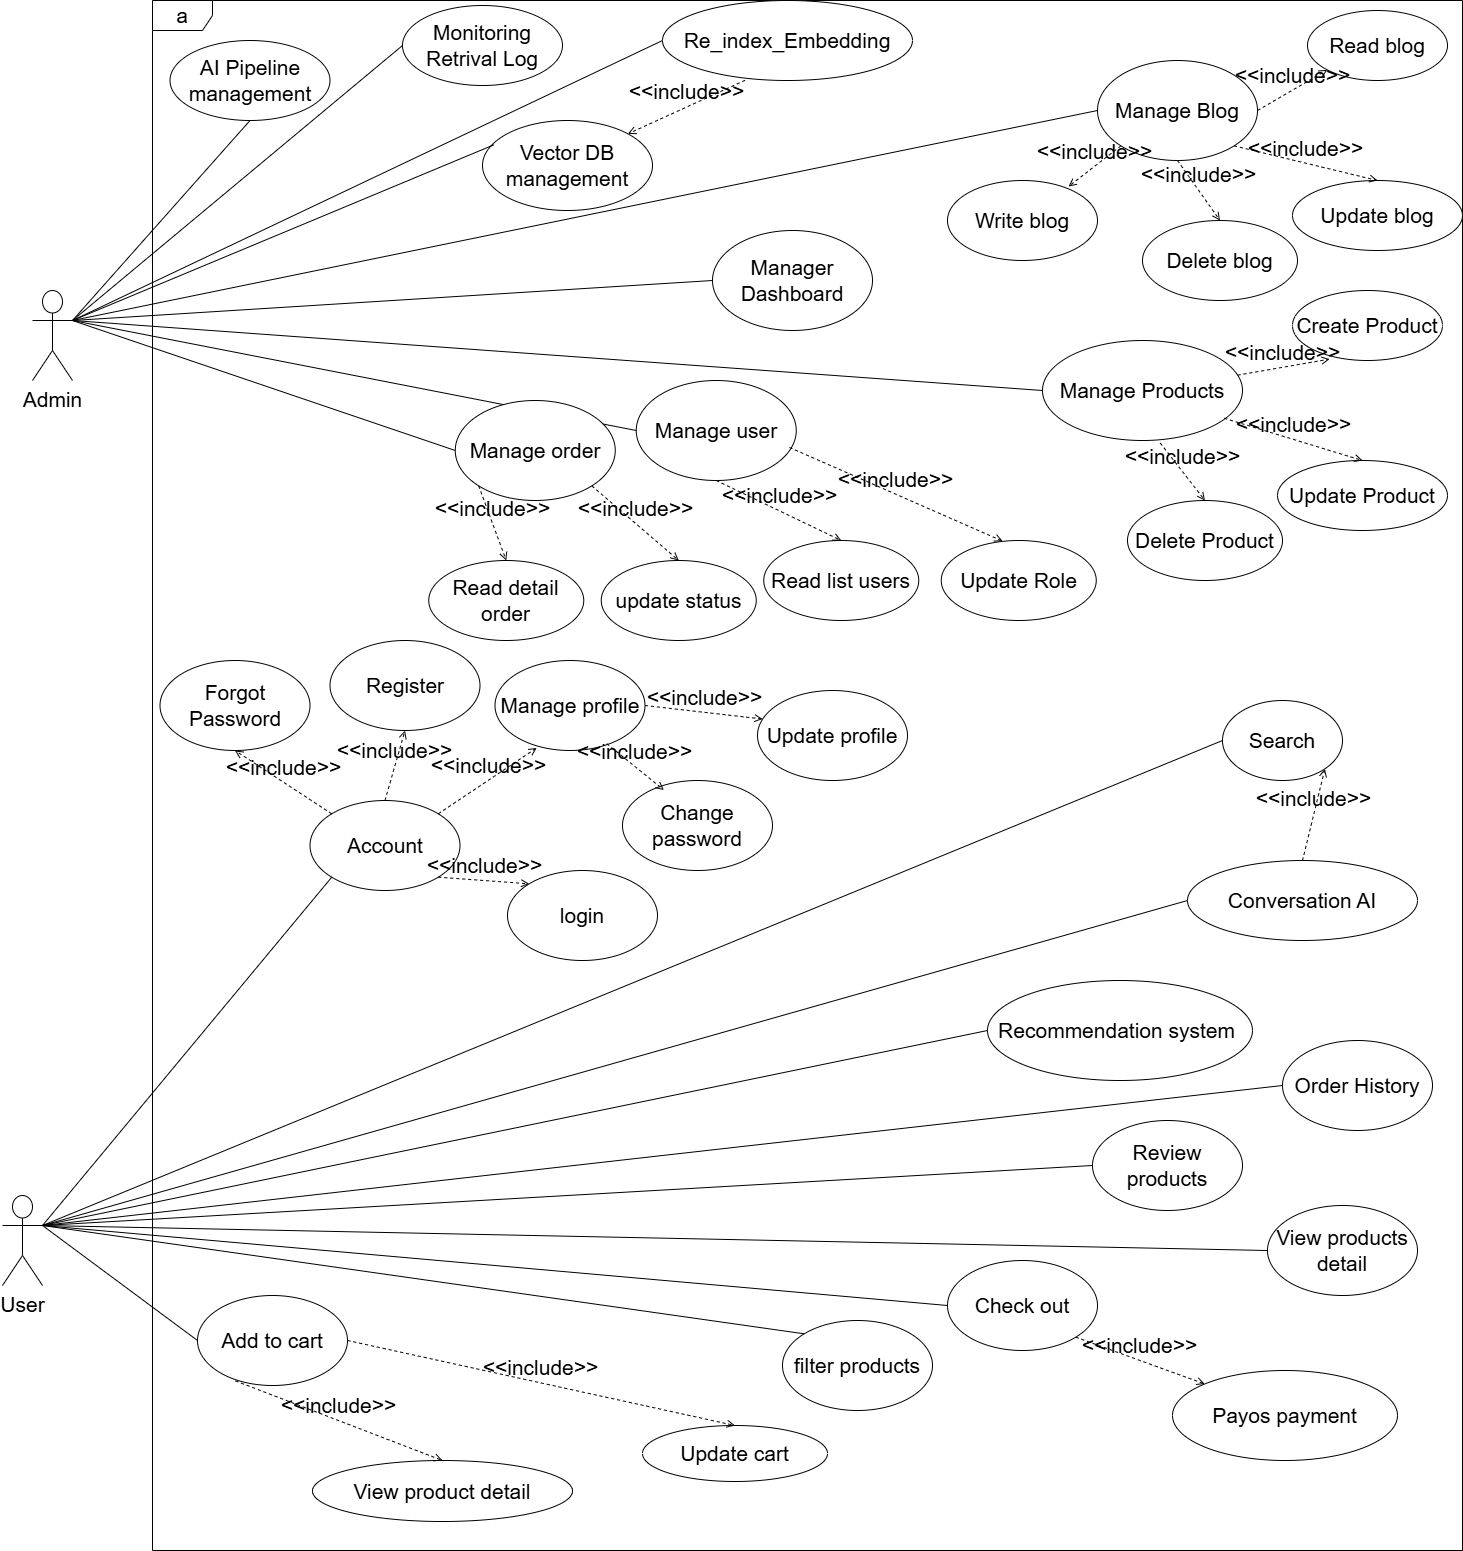
\includegraphics[width=0.9\linewidth]{Images/Usecase/usecase_DACN-Page-1.drawio.png}
%     \caption{Usecase toàn bộ hệ thống}
%     \label{fig:usecase-overall}
% \end{figure}



% Như trình bày ở Hình~\ref{fig:usecase-overall}, hệ thống thương mại điện tử AI bao gồm hai nhóm chức năng chính dành cho khách hàng và quản trị viên.

% Khách hàng có thể thực hiện các chức năng như đăng ký tài khoản, tìm kiếm sản phẩm, sử dụng AI Assistant để nhận tư vấn, xem sản phẩm gợi ý, thêm sản phẩm vào giỏ hàng, thanh toán và đánh giá sản phẩm.

% Quản trị viên chịu trách nhiệm quản lý dữ liệu hệ thống bao gồm quản lý sản phẩm, quản lý blog, quản lý người dùng, quản lý đơn hàng và quản lý AI Pipeline. Ngoài ra, hệ thống còn hỗ trợ Vector Database Management và Re-index Embedding để phục vụ cho chức năng tìm kiếm ngữ nghĩa và recommendation system.

% \subsubsection{Biểu đồ Use Case dành cho khách hàng}

% \begin{figure}[H]
%     \centering
%     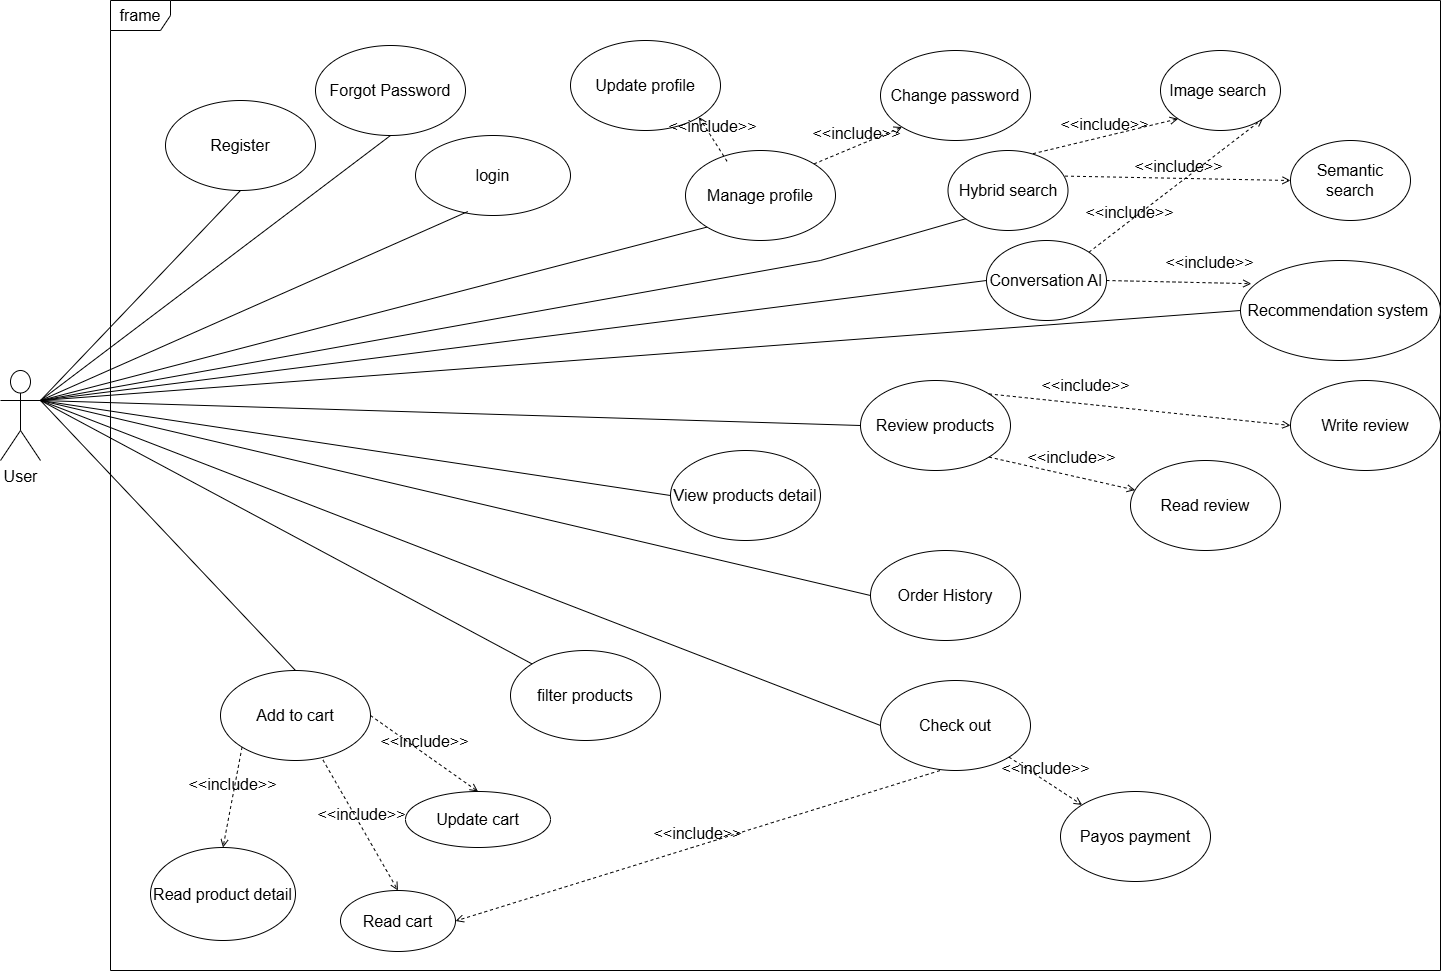
\includegraphics[width=0.9\linewidth]{Images/Usecase/usecase_DACN-Page-2.drawio.png}
%     \caption{Biểu đồ use case dành cho khách hàng}
%     \label{fig:usecase-customer}
% \end{figure}

% Như trình bày ở Hình~\ref{fig:usecase-user}, khách hàng có thể sử dụng các chức năng chính của hệ thống thương mại điện tử AI bao gồm quản lý tài khoản, tìm kiếm sản phẩm, sử dụng AI Assistant và thực hiện mua sắm trực tuyến.

% Hệ thống hỗ trợ nhiều phương thức tìm kiếm khác nhau như Semantic Search, Hybrid Search và Image Search nhằm nâng cao khả năng tìm kiếm sản phẩm theo nhu cầu người dùng.

% Ngoài ra, khách hàng có thể:
% \begin{itemize}
%     \item Đăng ký và đăng nhập hệ thống.
%     \item Quản lý hồ sơ cá nhân.
%     \item Thay đổi mật khẩu và cập nhật thông tin cá nhân.
%     \item Xem chi tiết sản phẩm.
%     \item Thêm sản phẩm vào giỏ hàng.
%     \item Cập nhật giỏ hàng.
%     \item Thanh toán đơn hàng thông qua cổng thanh toán PayOS.
%     \item Xem lịch sử đơn hàng.
%     \item Đánh giá sản phẩm sau khi mua.
%     \item Nhận gợi ý sản phẩm từ Recommendation System.
%     \item Tương tác với Conversation AI để nhận tư vấn mua sắm.
% \end{itemize}

% Trong đó, chức năng Hybrid Search bao gồm Semantic Search và Image Search nhằm hỗ trợ tìm kiếm sản phẩm bằng cả văn bản và hình ảnh. Recommendation System được tích hợp cùng Conversation AI để đề xuất các sản phẩm phù hợp với nhu cầu của khách hàng.

% \subsubsection{Biểu đồ Use Case dành cho quản trị viên}

% \begin{figure}[H]
%     \centering
%     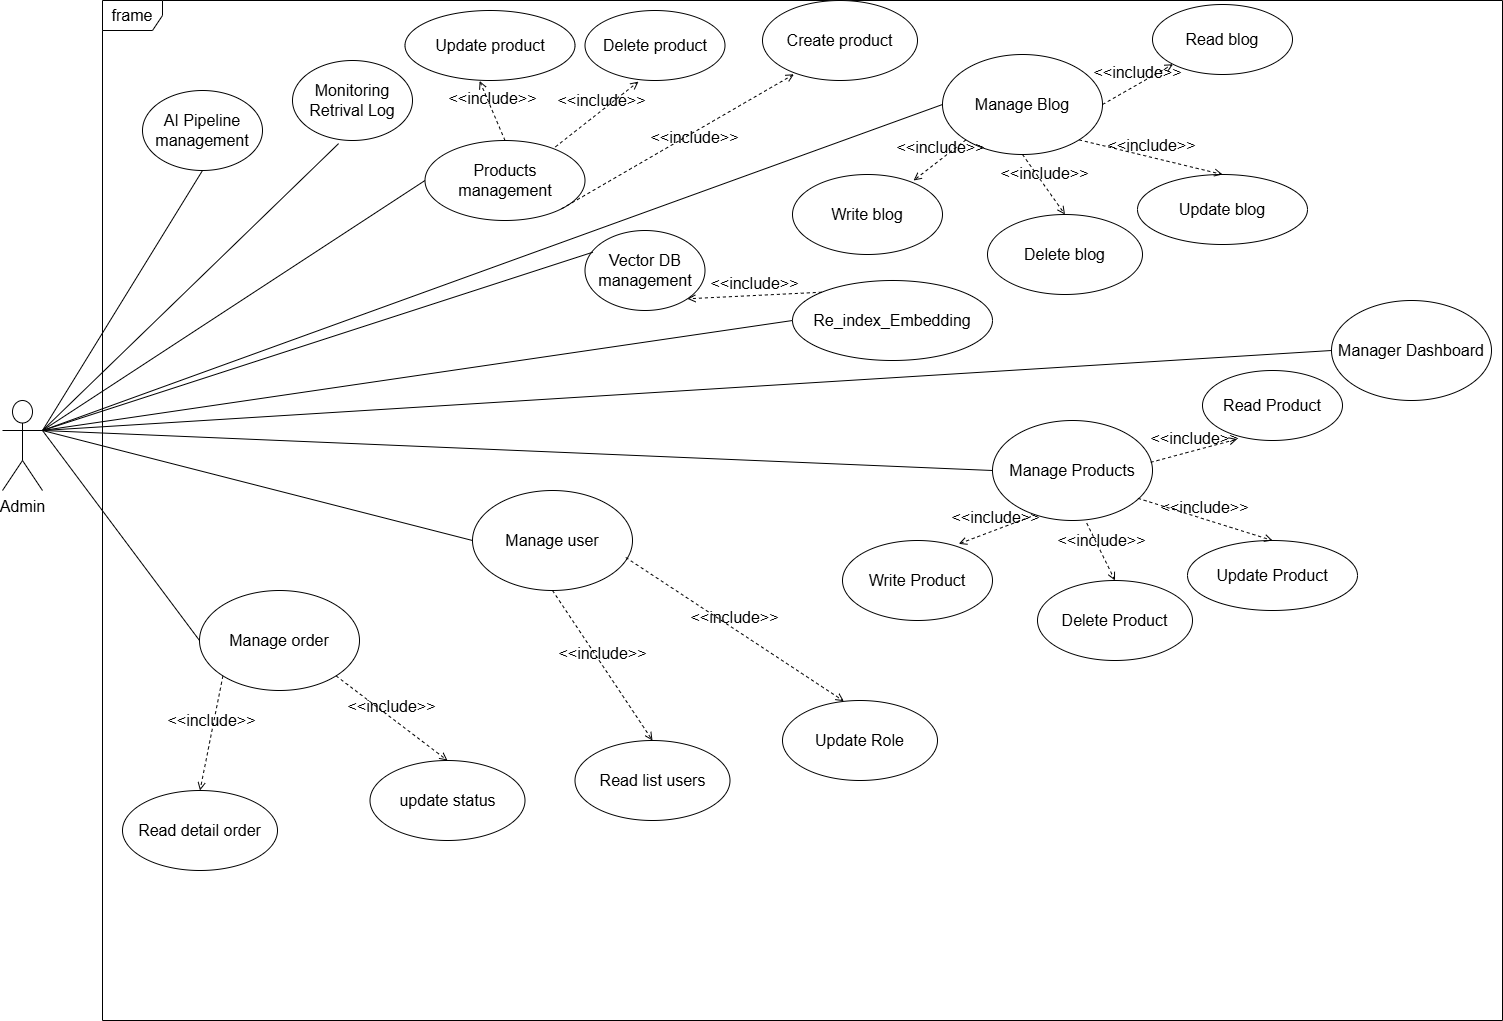
\includegraphics[width=0.9\linewidth]{Images/Usecase/usecase_DACN-Page-3.drawio.png}
%     \caption{Biểu đồ use case dành cho quản trị viên}
%     \label{fig:usecase-admin}
% \end{figure}

% Như trình bày ở Hình~\ref{fig:usecase-admin}, quản trị viên là tác nhân chịu trách nhiệm quản lý toàn bộ dữ liệu và hoạt động của hệ thống thương mại điện tử AI.

% Các chức năng chính của quản trị viên bao gồm:

% \begin{itemize}
%     \item Quản lý sản phẩm.
%     \item Quản lý người dùng.
%     \item Quản lý đơn hàng.
%     \item Quản lý blog.
%     \item Theo dõi dashboard hệ thống.
%     \item Quản lý AI Pipeline.
%     \item Theo dõi Monitoring Retrieval Log.
%     \item Quản lý Vector Database.
%     \item Thực hiện Re-index Embedding.
% \end{itemize}

% Trong chức năng quản lý sản phẩm, quản trị viên có thể thêm, sửa, xóa và xem danh sách sản phẩm.

% Đối với quản lý blog, hệ thống hỗ trợ tạo bài viết mới, chỉnh sửa bài viết, xóa bài viết và xem danh sách blog.

% Ngoài các chức năng quản trị thông thường, hệ thống còn hỗ trợ các chức năng liên quan đến AI như quản lý Vector Database và Re-index Embedding nhằm cập nhật dữ liệu embedding phục vụ cho Semantic Search, Recommendation System và Conversation AI.

% \subsubsection{Danh sách tác nhân}

% \begin{table}[H]
% \centering
% \caption{Danh sách tác nhân trong use case diagram}
% \label{tab:usecase-actors}
% \begin{tabularx}{\linewidth}{@{}p{0.25\linewidth}X@{}}
% \toprule
% \textbf{Tác nhân} & \textbf{Mô tả} \\
% \midrule
% Khách hàng & Người sử dụng hệ thống để tìm kiếm sản phẩm, nhận tư vấn từ assistant, xem sản phẩm gợi ý và lọc sản phẩm theo nhu cầu. \\
% Quản trị viên & Người quản lý sản phẩm và dữ liệu AI của hệ thống, có quyền thêm, xóa, sửa sản phẩm, đồng bộ dữ liệu sang AI Index và kiểm tra các tính năng liên quan đến AI Service. \\
% \bottomrule
% \end{tabularx}
% \end{table}


% % \end{table}

% \subsubsection{Mô tả các use case chính}

% \begin{table}[H]
% \centering
% \caption{Mô tả use case UC-US-01: Đăng nhập hệ thống}
% \label{tab:uc-login}
% \begin{tabularx}{\linewidth}{@{}p{0.28\linewidth}X@{}}
% \toprule
% \textbf{Thuộc tính} & \textbf{Mô tả} \\
% \midrule
% Mã use case & UC-US-01 \\
% Tên use case & Đăng nhập hệ thống \\
% Tác nhân & Khách hàng \\
% Tiền điều kiện & Người dùng đã có tài khoản trong hệ thống. \\
% Luồng chính &
% {
%  1/ Người dùng truy cập trang đăng nhập.

%  2/ Người dùng nhập email và mật khẩu.

%  3/ Hệ thống kiểm tra thông tin đăng nhập.

%  4/ Hệ thống xác thực thành công và chuyển đến trang chính.
% } \\
% Ngoại lệ &
% {
% 1/ Sai email hoặc mật khẩu.

% 2/ Tài khoản chưa được kích hoạt.
%  }\\
% Hậu điều kiện & Người dùng đăng nhập thành công vào hệ thống. \\
% \bottomrule
% \end{tabularx}
% \end{table}




% \begin{table}[H]
% \centering
% \caption{Mô tả use case UC-US-02: Hybrid Search sản phẩm}
% \label{tab:uc-hybrid-search}
% \begin{tabularx}{\linewidth}{@{}p{0.28\linewidth}X@{}}
% \toprule
% \textbf{Thuộc tính} & \textbf{Mô tả} \\
% \midrule
% Mã use case & UC-US-02 \\
% Tên use case & Hybrid Search sản phẩm \\
% Tác nhân & Khách hàng \\
% Tiền điều kiện & Người dùng truy cập hệ thống tìm kiếm sản phẩm. \\
% Luồng chính &
% {
% 1/ Người dùng nhập nội dung tìm kiếm hoặc tải ảnh sản phẩm.

% 2/ Hệ thống gửi yêu cầu đến AI Search Server.

% 3/ AI Service thực hiện Semantic Search và Image Search.

% 4/ Hệ thống tổng hợp kết quả tìm kiếm.

% 5/ Danh sách sản phẩm phù hợp được hiển thị cho người dùng.
% } \\
% Ngoại lệ &
% {
% 1/Không tìm thấy sản phẩm phù hợp.

% 2/AI Service không phản hồi.
% } \\
% Hậu điều kiện & Người dùng nhận được danh sách sản phẩm phù hợp với nhu cầu tìm kiếm. \\
% \bottomrule
% \end{tabularx}
% \end{table}




% \begin{table}[H]
% \centering
% \caption{Mô tả use case UC-US-03: Chat với Conversation AI}
% \label{tab:uc-conversation-ai}
% \begin{tabularx}{\linewidth}{@{}p{0.28\linewidth}X@{}}
% \toprule
% \textbf{Thuộc tính} & \textbf{Mô tả} \\
% \midrule
% Mã use case & UC-US-03 \\
% Tên use case & Chat với Conversation AI \\
% Tác nhân & Khách hàng \\
% Tiền điều kiện & Người dùng truy cập giao diện chat AI Assistant. \\
% Luồng chính &
% {
% 1/ Người dùng nhập câu hỏi hoặc nhu cầu mua sắm.

% 2/ Hệ thống gửi nội dung đến AI Service.

% 3/ Conversation AI xử lý yêu cầu.

% 4/ Recommendation System đề xuất sản phẩm phù hợp.

% 5/ Hệ thống hiển thị câu trả lời và danh sách sản phẩm gợi ý.
% } \\
% Ngoại lệ &
% {
%  1/ Nội dung không hợp lệ.

%  2/ AI Service không phản hồi.
% } \\
% Hậu điều kiện & Người dùng nhận được câu trả lời và sản phẩm gợi ý từ AI Assistant. \\
% \bottomrule
% \end{tabularx}
% \end{table}


% \begin{table}[H]
% \centering
% \caption{Mô tả use case UC-US-04: Thêm sản phẩm vào giỏ hàng}
% \label{tab:uc-add-cart}
% \begin{tabularx}{\linewidth}{@{}p{0.28\linewidth}X@{}}
% \toprule
% \textbf{Thuộc tính} & \textbf{Mô tả} \\
% \midrule
% Mã use case & UC-US-04 \\
% Tên use case & Thêm sản phẩm vào giỏ hàng \\
% Tác nhân & Khách hàng \\
% Tiền điều kiện & Người dùng đang xem chi tiết sản phẩm. \\
% Luồng chính &
% \begin{enumerate}
%     \item Người dùng chọn số lượng sản phẩm.
%     \item Người dùng nhấn nút thêm vào giỏ hàng.
%     \item Hệ thống kiểm tra tồn kho sản phẩm.
%     \item Hệ thống cập nhật giỏ hàng.
% \end{enumerate} \\
% Ngoại lệ &
% \begin{itemize}
%     \item Sản phẩm hết hàng.
%     \item Người dùng chưa đăng nhập.
% \end{itemize} \\
% Hậu điều kiện & Sản phẩm được thêm vào giỏ hàng thành công. \\
% \bottomrule
% \end{tabularx}
% \end{table}



% \begin{table}[H]
% \centering
% \caption{Mô tả use case UC-KH-03: Xem sản phẩm gợi ý}
% \label{tab:uc-product-suggestion}
% \begin{tabularx}{\linewidth}{@{}p{0.25\linewidth}X@{}}
% \toprule
% \textbf{Thuộc tính} & \textbf{Mô tả} \\
% \midrule
% Mã use case & UC-KH-03 \\
% Tên use case & Xem sản phẩm gợi ý \\
% Tác nhân & Khách hàng \\
% Tiền điều kiện & Hệ thống đã có danh sách sản phẩm gợi ý từ kết quả tìm kiếm hoặc từ assistant. \\
% Luồng chính & Hệ thống lấy danh sách sản phẩm gợi ý; hệ thống lấy thông tin chi tiết của từng sản phẩm; hệ thống hiển thị sản phẩm dưới dạng danh sách hoặc thẻ sản phẩm; khách hàng xem thông tin sản phẩm được đề xuất. \\
% Ngoại lệ & Sản phẩm gợi ý không còn tồn tại, đã hết hàng hoặc không khả dụng. \\
% Hậu điều kiện & Khách hàng xem được danh sách sản phẩm được đề xuất. \\
% \bottomrule
% \end{tabularx}
% \end{table}




% \begin{table}[H]
% \centering
% \caption{Mô tả use case UC-AD-01: Thêm xóa sửa sản phẩm}
% \label{tab:uc-admin-crud-product}
% \begin{tabularx}{\linewidth}{@{}p{0.25\linewidth}X@{}}
% \toprule
% \textbf{Thuộc tính} & \textbf{Mô tả} \\
% \midrule
% Mã use case & UC-AD-01 \\
% Tên use case & Thêm xóa sửa sản phẩm \\
% Tác nhân & Quản trị viên \\
% Tiền điều kiện & Quản trị viên đã đăng nhập vào hệ thống và có quyền quản lý sản phẩm. \\
% Luồng chính & Quản trị viên truy cập chức năng quản lý sản phẩm; quản trị viên chọn thao tác thêm, xóa hoặc sửa sản phẩm; hệ thống hiển thị biểu mẫu hoặc thông tin sản phẩm; quản trị viên nhập hoặc cập nhật thông tin; hệ thống kiểm tra dữ liệu và lưu thay đổi. \\
% Ngoại lệ & Dữ liệu sản phẩm không hợp lệ, thiếu thông tin bắt buộc hoặc thao tác cập nhật thất bại. \\
% Hậu điều kiện & Thông tin sản phẩm trong hệ thống được thêm mới, cập nhật hoặc xóa theo thao tác của quản trị viên. \\
% \bottomrule
% \end{tabularx}
% \end{table}


% \begin{table}[H]
% \centering
% \caption{Mô tả use case UC-US-04: Thêm sản phẩm vào giỏ hàng}
% \label{tab:uc-add-cart}
% \begin{tabularx}{\linewidth}{@{}p{0.28\linewidth}X@{}}
% \toprule
% \textbf{Thuộc tính} & \textbf{Mô tả} \\
% \midrule
% Mã use case & UC-US-04 \\
% Tên use case & Thêm sản phẩm vào giỏ hàng \\
% Tác nhân & Khách hàng \\
% Tiền điều kiện & Người dùng đang xem chi tiết sản phẩm. \\
% Luồng chính &
% \begin{enumerate}
%     \item Người dùng chọn số lượng sản phẩm.
%     \item Người dùng nhấn nút thêm vào giỏ hàng.
%     \item Hệ thống kiểm tra tồn kho sản phẩm.
%     \item Hệ thống cập nhật giỏ hàng.
% \end{enumerate} \\
% Ngoại lệ &
% \begin{itemize}
%     \item Sản phẩm hết hàng.
%     \item Người dùng chưa đăng nhập.
% \end{itemize} \\
% Hậu điều kiện & Sản phẩm được thêm vào giỏ hàng thành công. \\
% \bottomrule
% \end{tabularx}
% \end{table}




% \begin{table}[H]
% \centering
% \caption{Mô tả use case UC-US-05: Thanh toán đơn hàng}
% \label{tab:uc-checkout}
% \begin{tabularx}{\linewidth}{@{}p{0.28\linewidth}X@{}}
% \toprule
% \textbf{Thuộc tính} & \textbf{Mô tả} \\
% \midrule
% Mã use case & UC-US-05 \\
% Tên use case & Thanh toán đơn hàng \\
% Tác nhân & Khách hàng \\
% Tiền điều kiện & Giỏ hàng có ít nhất một sản phẩm. \\
% Luồng chính &
% \begin{enumerate}
%     \item Người dùng truy cập trang checkout.
%     \item Hệ thống hiển thị thông tin đơn hàng.
%     \item Người dùng nhập thông tin giao hàng.
%     \item Người dùng chọn phương thức thanh toán.
%     \item Hệ thống chuyển sang cổng thanh toán PayOS.
%     \item Thanh toán thành công.
% \end{enumerate} \\
% Ngoại lệ &
% \begin{itemize}
%     \item Thanh toán thất bại.
%     \item Người dùng hủy giao dịch.
% \end{itemize} \\
% Hậu điều kiện & Đơn hàng được tạo thành công trong hệ thống. \\
% \bottomrule
% \end{tabularx}
% \end{table}

\subsection{Phân tích ca sử dụng}

Phần này đặc tả chi tiết các ca sử dụng có luồng giao dịch, chuyển trạng thái hoặc xử lý AI đặc trưng. Các thao tác còn lại được tổng hợp theo nhóm để bảo đảm khả năng truy vết mà không lặp lại nội dung đã thể hiện trên biểu đồ và các sơ đồ hành vi.

\newcommand{\UseCaseSpecification}[7]{%
    \begin{table}[!htbp]
        \centering
        \caption{Đặc tả #1 -- #2}
        \begin{tabularx}{\textwidth}{|p{0.25\textwidth}|X|}
            \hline
            \textbf{Tác nhân} & #3 \\ \hline
            \textbf{Tiền điều kiện và kích hoạt} & #4 \\ \hline
            \textbf{Luồng chính} & #5 \\ \hline
            \textbf{Luồng thay thế/ngoại lệ} & #6 \\ \hline
            \textbf{Hậu điều kiện} & #7 \\ \hline
        \end{tabularx}
    \end{table}
}

\subsubsection{Tác nhân của hệ thống}

\begin{table}[!htbp]
    \centering
    \caption{Các tác nhân tham gia hệ thống}
    \label{tab:usecase-actors}
    \begin{tabularx}{\textwidth}{|p{0.22\textwidth}|X|}
        \hline
        \textbf{Tác nhân} & \textbf{Vai trò} \\ \hline
        Khách vãng lai & Tra cứu sản phẩm, bài viết và sử dụng các chức năng tìm kiếm công khai. \\ \hline
        Khách hàng & Quản lý tài khoản, giỏ hàng, đơn hàng và tương tác với trợ lý AI. \\ \hline
        Quản trị viên & Quản trị danh mục, sản phẩm, tồn kho, đơn hàng, nội dung và vận hành dữ liệu AI. \\ \hline
        Dịch vụ AI & Thực hiện tìm kiếm ngữ nghĩa, tìm kiếm ảnh/kết hợp, hội thoại RAG và quản lý chỉ mục vector. \\ \hline
    \end{tabularx}
\end{table}

\subsubsection{Ca sử dụng của khách hàng}

\begin{figure}[!htbp]
    \centering
    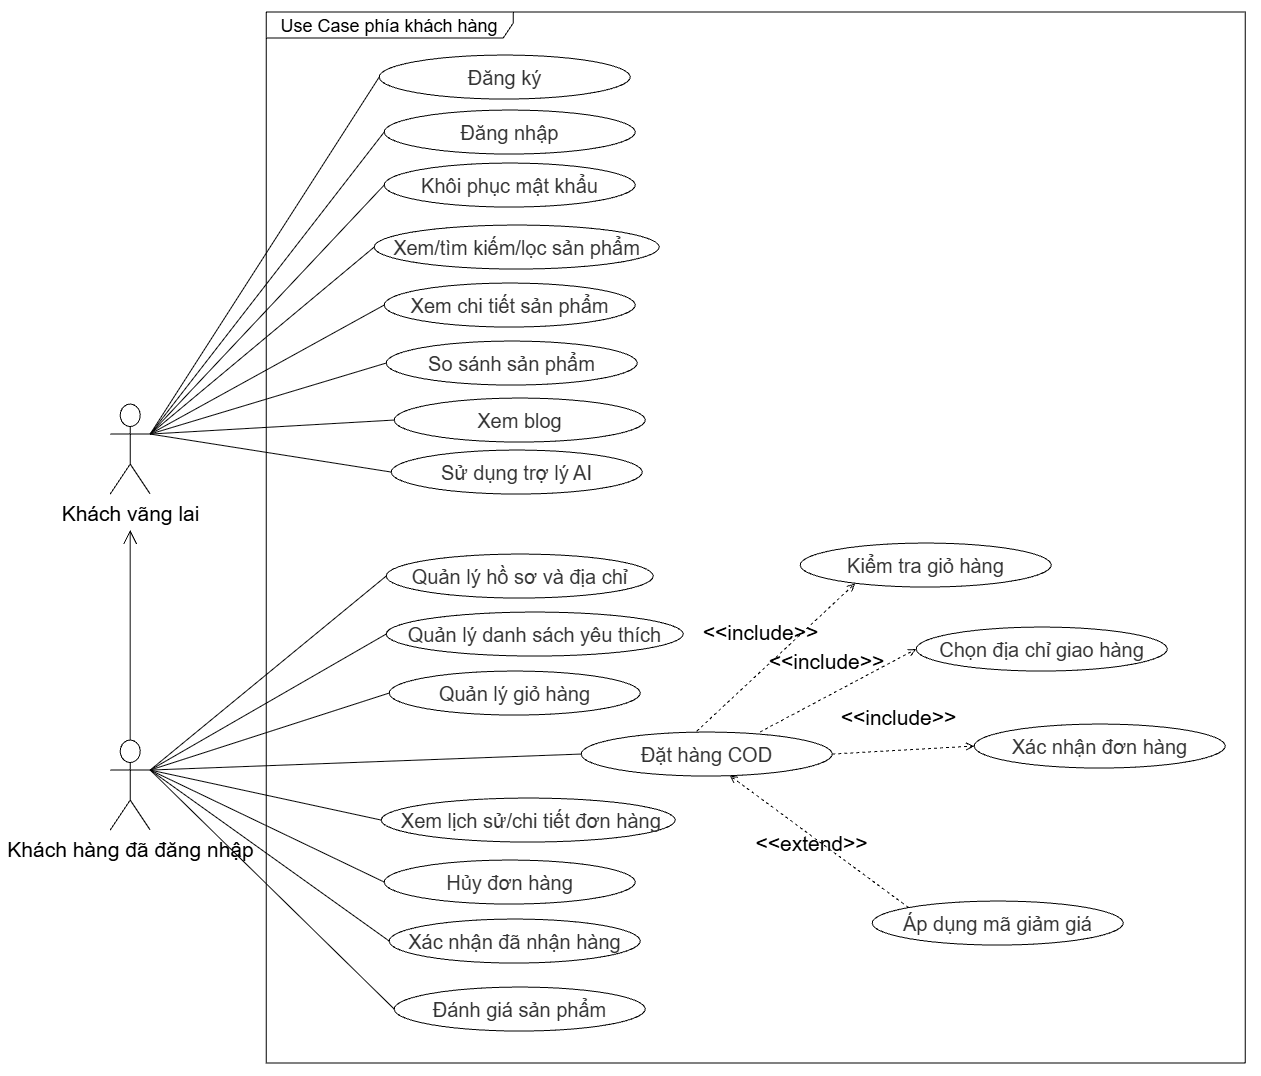
\includegraphics[width=0.94\textwidth]{Images/Usecase/da-Use Case phía khách hàng.drawio.png}
    \caption{Biểu đồ ca sử dụng phía khách hàng}
    \label{fig:usecase-customer}
\end{figure}

\begin{longtable}{|p{0.10\textwidth}|p{0.18\textwidth}|p{0.15\textwidth}|p{0.20\textwidth}|p{0.24\textwidth}|}
    \caption{Danh mục ca sử dụng phía khách hàng}\label{tab:usecase-customer-summary}\\
    \hline
    \textbf{Mã} & \textbf{Tên ca sử dụng} & \textbf{Tác nhân} & \textbf{Mục tiêu} & \textbf{Điều kiện/Kết quả chính} \\ \hline
    \endfirsthead
    \hline
    \textbf{Mã} & \textbf{Tên ca sử dụng} & \textbf{Tác nhân} & \textbf{Mục tiêu} & \textbf{Điều kiện/Kết quả chính} \\ \hline
    \endhead
    UC-KH-01 & Đăng ký & Khách vãng lai & Tạo tài khoản mới & Thông tin hợp lệ; tài khoản được tạo và xác thực. \\ \hline
    UC-KH-02 & Đăng nhập & Khách vãng lai & Truy cập chức năng cá nhân & Thông tin đúng; phiên đăng nhập được thiết lập. \\ \hline
    UC-KH-03 & Khôi phục mật khẩu & Khách vãng lai & Cấp lại quyền truy cập & Email tồn tại; mật khẩu được đặt lại an toàn. \\ \hline
    UC-KH-04 & Xem danh mục & Mọi khách hàng & Duyệt danh mục sản phẩm & Danh mục khả dụng; danh sách được hiển thị. \\ \hline
    UC-KH-05 & Tìm kiếm truyền thống & Mọi khách hàng & Tìm theo từ khóa và bộ lọc & Truy vấn hợp lệ; trả về sản phẩm phù hợp. \\ \hline
    UC-KH-06 & Xem chi tiết sản phẩm & Mọi khách hàng & Xem biến thể, giá và tồn kho & Sản phẩm còn hoạt động; dữ liệu hiện hành được hiển thị. \\ \hline
    UC-KH-07 & So sánh sản phẩm & Mọi khách hàng & Đối chiếu thuộc tính & Có các sản phẩm hợp lệ; bảng so sánh được tạo. \\ \hline
    UC-KH-08 & Xem bài viết & Mọi khách hàng & Tra cứu nội dung tư vấn & Bài viết đã xuất bản; nội dung được hiển thị. \\ \hline
    UC-KH-09 & Quản lý hồ sơ, địa chỉ và yêu thích & Khách hàng & Cập nhật dữ liệu cá nhân & Đã đăng nhập; dữ liệu được lưu đúng quyền sở hữu. \\ \hline
    UC-KH-10 & Quản lý giỏ hàng & Khách hàng & Thêm, sửa, xóa sản phẩm & Biến thể hợp lệ; giỏ phản ánh giá và tồn kho hiện hành. \\ \hline
    UC-KH-11 & Đặt hàng COD & Khách hàng & Tạo đơn thanh toán khi nhận hàng & Giỏ và địa chỉ hợp lệ; đơn COD được tạo. \\ \hline
    UC-KH-12 & Xem lịch sử đơn hàng & Khách hàng & Theo dõi đơn đã đặt & Đã đăng nhập; chỉ hiển thị đơn thuộc khách hàng. \\ \hline
    UC-KH-13 & Hủy đơn hàng & Khách hàng & Hủy đơn còn cho phép & Đơn đúng chủ và đúng trạng thái; tồn kho được hoàn trả. \\ \hline
    UC-KH-14 & Xác nhận nhận hàng & Khách hàng & Hoàn tất đơn đã giao & Đơn đang giao; trạng thái được chuyển hoàn tất. \\ \hline
    UC-KH-15 & Đánh giá sản phẩm & Khách hàng & Gửi nhận xét sau mua & Đơn đã hoàn tất; đánh giá được ghi nhận để kiểm duyệt. \\ \hline
    UC-KH-16 & Sử dụng trợ lý AI & Mọi khách hàng & Truy cập nhóm chức năng AI & Yêu cầu hợp lệ; chuyển tới ca sử dụng AI tương ứng. \\ \hline
\end{longtable}

\UseCaseSpecification{UC-KH-10}{Quản lý giỏ hàng}
{Khách hàng đã đăng nhập}
{Biến thể sản phẩm đang hoạt động; khách hàng thêm sản phẩm hoặc thay đổi số lượng trong giỏ.}
{Hệ thống lấy giỏ hiện tại, kiểm tra biến thể, giá và tồn kho; sau đó thêm, cập nhật hoặc xóa dòng hàng và tính lại tổng tiền.}
{Số lượng bằng không được hiểu là xóa; từ chối khi biến thể không hợp lệ, vượt tồn kho hoặc giỏ không thuộc khách hàng.}
{Giỏ hàng nhất quán với giá, biến thể và số lượng có thể bán tại thời điểm cập nhật.}

\UseCaseSpecification{UC-KH-11}{Đặt hàng COD}
{Khách hàng đã đăng nhập}
{Giỏ có sản phẩm hợp lệ và còn hàng; khách hàng đã chọn địa chỉ rồi xác nhận thanh toán COD.}
{Hệ thống kiểm tra lại giỏ và tồn kho, áp dụng mã giảm giá nếu có, tính tổng tiền, tạo đơn cùng chi tiết đơn và bản ghi thanh toán COD.}
{Khách hàng có thể bỏ mã giảm giá; hệ thống dừng khi giỏ rỗng, hết hàng, địa chỉ hoặc mã không hợp lệ, hay giao dịch tạo đơn thất bại.}
{Đơn COD được tạo một lần, dữ liệu giá được chốt và tồn kho được cập nhật theo quy tắc nghiệp vụ.}

\UseCaseSpecification{UC-KH-13}{Hủy đơn hàng}
{Khách hàng đã đăng nhập}
{Đơn thuộc khách hàng và đang ở trạng thái cho phép hủy; khách hàng gửi yêu cầu hủy.}
{Hệ thống khóa và kiểm tra đơn, chuyển trạng thái sang đã hủy, hoàn phần tồn kho liên quan và ghi lịch sử thay đổi.}
{Từ chối nếu đơn không thuộc khách hàng, đã qua giai đoạn cho phép hủy hoặc vừa được tiến trình khác cập nhật.}
{Đơn ở trạng thái đã hủy; tồn kho và lịch sử trạng thái được cập nhật nhất quán.}

\subsubsection{Ca sử dụng của quản trị viên}

\begin{figure}[!htbp]
    \centering
    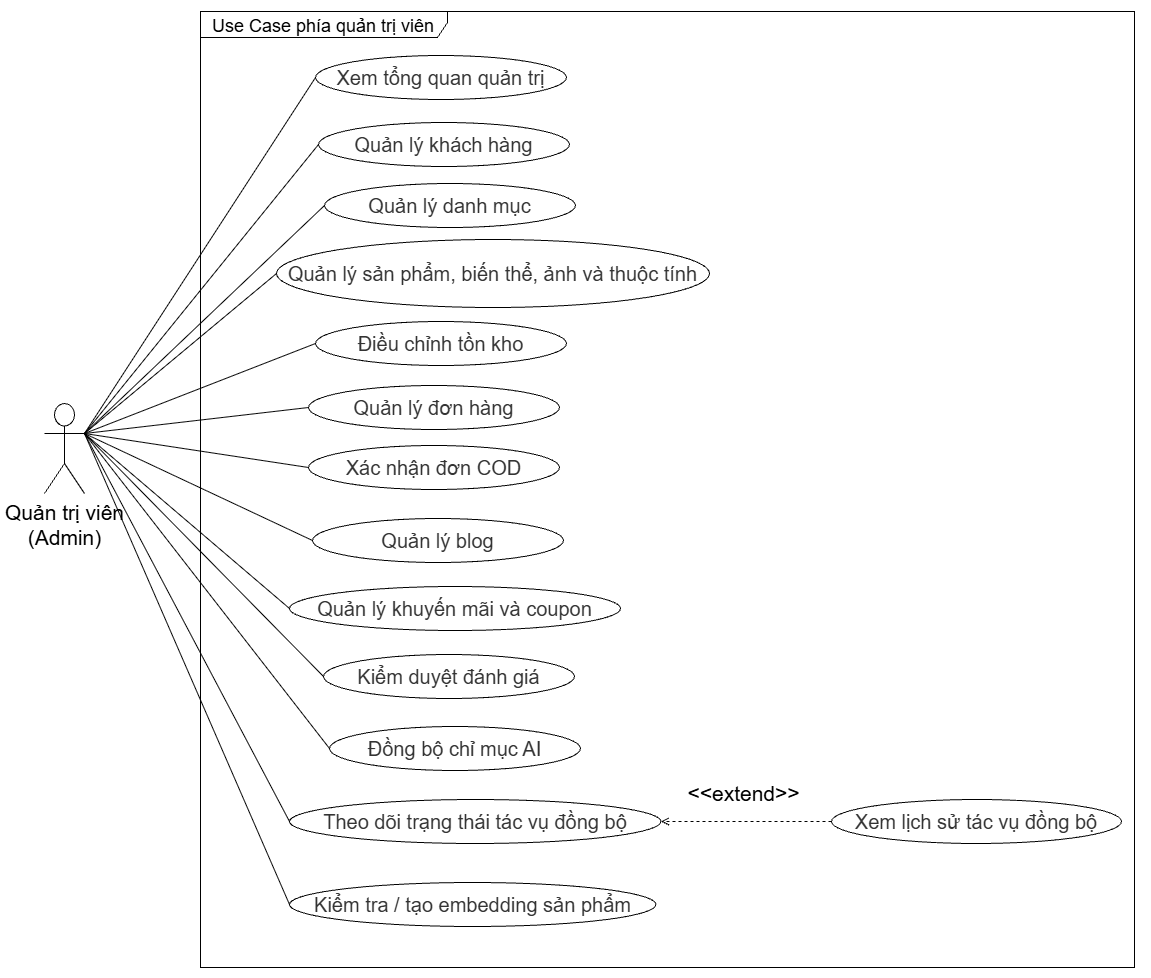
\includegraphics[width=0.92\textwidth]{Images/Usecase/da-Use Case phía quản trị viên.drawio.png}
    \caption{Biểu đồ ca sử dụng phía quản trị viên}
    \label{fig:usecase-admin}
\end{figure}

\begin{longtable}{|p{0.10\textwidth}|p{0.18\textwidth}|p{0.15\textwidth}|p{0.20\textwidth}|p{0.24\textwidth}|}
    \caption{Danh mục ca sử dụng phía quản trị viên}\label{tab:usecase-admin-summary}\\
    \hline
    \textbf{Mã} & \textbf{Tên ca sử dụng} & \textbf{Tác nhân} & \textbf{Mục tiêu} & \textbf{Điều kiện/Kết quả chính} \\ \hline
    \endfirsthead
    \hline
    \textbf{Mã} & \textbf{Tên ca sử dụng} & \textbf{Tác nhân} & \textbf{Mục tiêu} & \textbf{Điều kiện/Kết quả chính} \\ \hline
    \endhead
    UC-AD-01 & Xem dashboard & Quản trị viên & Theo dõi chỉ số vận hành & Có quyền truy cập; số liệu tổng hợp được hiển thị. \\ \hline
    UC-AD-02 & Quản lý khách hàng & Quản trị viên & Tra cứu và cập nhật trạng thái tài khoản & Có quyền quản trị; thay đổi được lưu và ghi nhận. \\ \hline
    UC-AD-03 & Quản lý danh mục & Quản trị viên & Tổ chức cây danh mục & Dữ liệu hợp lệ; cấu trúc danh mục được cập nhật. \\ \hline
    UC-AD-04 & Quản lý sản phẩm & Quản trị viên & Quản lý sản phẩm, biến thể và thuộc tính & Có quyền danh mục; dữ liệu được lưu và đánh dấu đồng bộ AI. \\ \hline
    UC-AD-05 & Điều chỉnh tồn kho & Quản trị viên & Điều chỉnh số lượng có thể bán & Biến thể tồn tại; tồn kho và lịch sử được cập nhật. \\ \hline
    UC-AD-06 & Quản lý đơn hàng & Quản trị viên & Tra cứu và xử lý vòng đời đơn & Có quyền đơn hàng; trạng thái tuân thủ quy tắc chuyển đổi. \\ \hline
    UC-AD-07 & Xác nhận đơn COD & Quản trị viên & Xác nhận đơn đủ điều kiện xử lý & Đơn COD và tồn kho hợp lệ; giao dịch được ghi nhận. \\ \hline
    UC-AD-08 & Quản lý bài viết & Quản trị viên & Soạn và xuất bản nội dung & Nội dung hợp lệ; trạng thái xuất bản được cập nhật. \\ \hline
    UC-AD-09 & Quản lý khuyến mãi & Quản trị viên & Cấu hình chương trình giảm giá & Điều kiện và thời gian hợp lệ; chương trình được lưu. \\ \hline
    UC-AD-10 & Kiểm duyệt đánh giá & Quản trị viên & Duyệt hoặc ẩn phản hồi & Có quyền kiểm duyệt; trạng thái đánh giá được cập nhật. \\ \hline
\end{longtable}

Các tác vụ vận hành AI trước đây ký hiệu UC-AD-11, UC-AD-12 và UC-AD-13 được quy về UC-AI-07, UC-AI-08 và UC-AI-09. Cách biểu diễn này giữ quan hệ quản trị viên khởi tạo tác vụ nhưng tránh đặc tả trùng lặp ở hai nhóm.

\UseCaseSpecification{UC-AD-04}{Quản lý sản phẩm}
{Quản trị viên có quyền quản lý danh mục}
{Sản phẩm hoặc danh mục liên quan tồn tại khi cập nhật; quản trị viên tạo mới hoặc chỉnh sửa sản phẩm.}
{Hệ thống kiểm tra dữ liệu chính, biến thể, ảnh và thuộc tính; lưu các thay đổi trong một giao dịch và đánh dấu dữ liệu cần đồng bộ sang chỉ mục AI.}
{Có thể cập nhật từng thành phần độc lập; từ chối SKU trùng, giá hoặc biến thể không hợp lệ, lỗi tải ảnh hay lỗi giao dịch.}
{Dữ liệu sản phẩm nhất quán và trạng thái đồng bộ AI được ghi nhận để xử lý tiếp.}

\UseCaseSpecification{UC-AD-07}{Xác nhận đơn COD}
{Quản trị viên có quyền xử lý đơn hàng}
{Đơn sử dụng COD, đang ở trạng thái có thể xác nhận và còn đủ tồn kho; quản trị viên chọn xác nhận.}
{Hệ thống khóa đơn, kiểm tra thanh toán và tồn kho, xác nhận đơn, cập nhật trạng thái liên quan, đồng thời ghi giao dịch kho và lịch sử xử lý.}
{Từ chối khi đơn không phải COD, thiếu tồn kho, đã được xử lý hoặc giao dịch cập nhật thất bại.}
{Đơn chuyển sang trạng thái xử lý kế tiếp; thanh toán, tồn kho và lịch sử trạng thái nhất quán.}

\subsubsection{Ca sử dụng của AI Service}

\begin{figure}[!htbp]
    \centering
    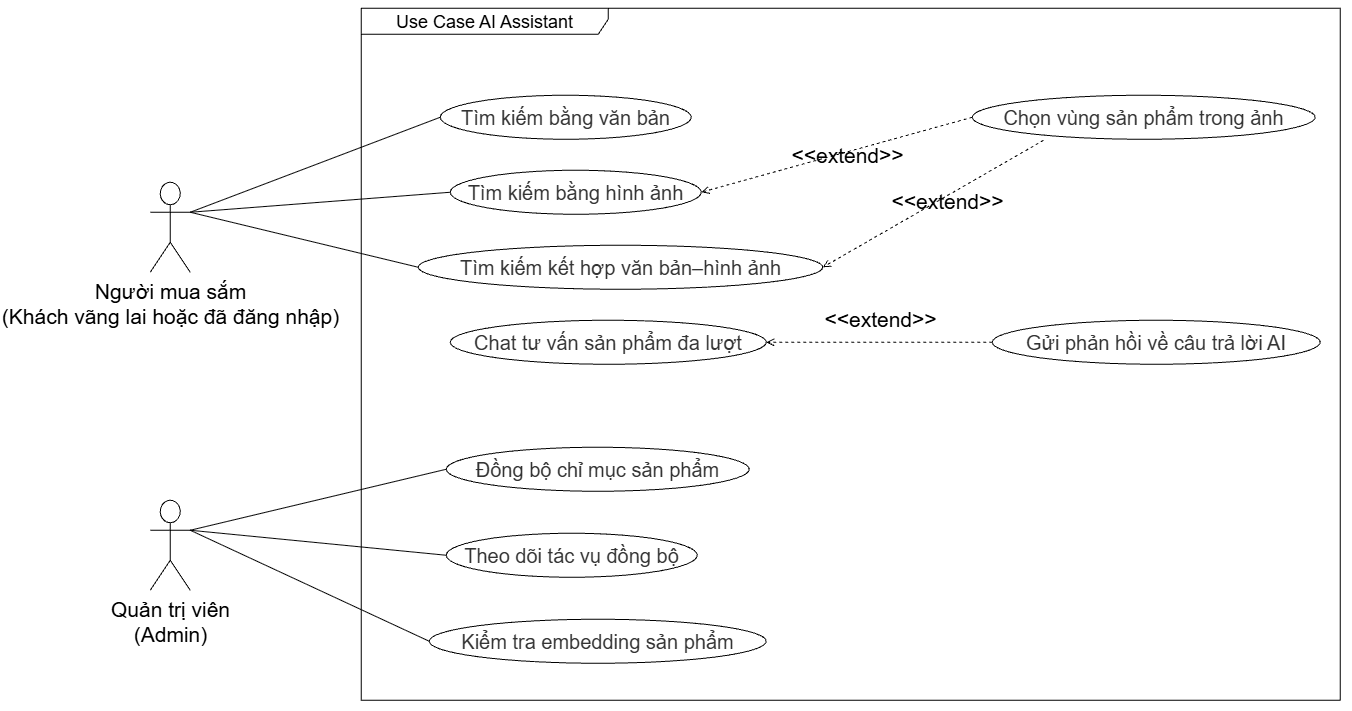
\includegraphics[width=\linewidth]{Images/Usecase/da-Use Case AI Assistant.drawio.png}
    \caption{Biểu đồ ca sử dụng của AI Service}
    \label{fig:usecase-ai-assistant}
\end{figure}

\begin{longtable}{|p{0.10\textwidth}|p{0.18\textwidth}|p{0.15\textwidth}|p{0.20\textwidth}|p{0.24\textwidth}|}
    \caption{Danh mục ca sử dụng của AI Service}\label{tab:usecase-ai-summary}\\
    \hline
    \textbf{Mã} & \textbf{Tên ca sử dụng} & \textbf{Tác nhân} & \textbf{Mục tiêu} & \textbf{Điều kiện/Kết quả chính} \\ \hline
    \endfirsthead
    \hline
    \textbf{Mã} & \textbf{Tên ca sử dụng} & \textbf{Tác nhân} & \textbf{Mục tiêu} & \textbf{Điều kiện/Kết quả chính} \\ \hline
    \endhead
    UC-AI-01 & Tìm kiếm văn bản & Người mua & Tìm sản phẩm theo ngữ nghĩa & Truy vấn hợp lệ; trả về danh sách đã xếp hạng. \\ \hline
    UC-AI-02 & Tìm kiếm hình ảnh & Người mua & Tìm sản phẩm tương tự ảnh & Ảnh hợp lệ và chỉ mục sẵn sàng; trả về kết quả tương tự. \\ \hline
    UC-AI-03 & Tìm kiếm kết hợp & Người mua & Kết hợp tín hiệu văn bản và ảnh & Có ít nhất một tín hiệu hợp lệ; kết quả được hợp nhất và xếp hạng. \\ \hline
    UC-AI-04 & Chat tư vấn đa lượt & Người mua & Nhận tư vấn dựa trên dữ liệu sản phẩm & Phiên hợp lệ; phản hồi có ngữ cảnh và được lưu vào hội thoại. \\ \hline
    UC-AI-05 & Chọn vùng ảnh & Người mua & Giới hạn đối tượng cần tìm & Vùng chọn hợp lệ; được xử lý như luồng mở rộng của UC-AI-02/03. \\ \hline
    UC-AI-06 & Gửi phản hồi AI & Khách hàng & Ghi nhận mức hữu ích của kết quả & Có kết quả hoặc hội thoại; phản hồi được lưu để đánh giá. \\ \hline
    UC-AI-07 & Đồng bộ chỉ mục & Quản trị viên & Cập nhật vector theo dữ liệu nghiệp vụ & Có quyền vận hành; tác vụ đồng bộ được tạo và thực thi. \\ \hline
    UC-AI-08 & Theo dõi tác vụ đồng bộ & Quản trị viên & Theo dõi tiến độ và lỗi & Có mã tác vụ; trạng thái và thống kê được hiển thị. \\ \hline
    UC-AI-09 & Kiểm tra embedding & Quản trị viên & Kiểm tra độ đầy đủ của chỉ mục & Chỉ mục truy cập được; báo cáo sai lệch được tạo. \\ \hline
\end{longtable}

\UseCaseSpecification{UC-AI-02}{Tìm kiếm hình ảnh}
{Người mua}
{Ảnh đúng định dạng, dung lượng cho phép và chỉ mục ảnh sẵn sàng; người mua tải ảnh hoặc chọn vùng ảnh để tìm kiếm.}
{Dịch vụ kiểm tra và giải mã ảnh, dùng ảnh gốc hoặc vùng chọn để sinh embedding, truy hồi và xếp hạng vector, rồi ánh xạ sang dữ liệu sản phẩm hiện hành.}
{Không chọn vùng thì dùng ảnh gốc hoặc vùng được phát hiện tự động; trả lỗi có kiểm soát khi ảnh hỏng, dịch vụ hoặc chỉ mục không sẵn sàng.}
{Danh sách sản phẩm tương tự, hoặc kết quả rỗng có giải thích, được trả về cho giao diện.}

\UseCaseSpecification{UC-AI-03}{Tìm kiếm kết hợp}
{Người mua}
{Có văn bản và ảnh hợp lệ, các chỉ mục liên quan sẵn sàng; người mua gửi yêu cầu tìm kiếm kết hợp.}
{Dịch vụ phân tích hai tín hiệu, truy hồi theo văn bản và ảnh, hợp nhất điểm, áp dụng bộ lọc, xếp hạng rồi lấy dữ liệu sản phẩm hiện hành.}
{Nếu một nhánh thất bại, hệ thống có thể dùng nhánh còn lại và kèm cảnh báo; yêu cầu thất bại khi cả hai tín hiệu không hợp lệ hoặc đều không khả dụng.}
{Kết quả phản ánh đồng thời ý định văn bản và mức tương đồng hình ảnh trong phạm vi dữ liệu đang bán.}

\UseCaseSpecification{UC-AI-04}{Chat tư vấn đa lượt}
{Người mua}
{Phiên hội thoại hợp lệ và nội dung gửi lên được chấp nhận; người mua đặt câu hỏi hoặc bổ sung ràng buộc.}
{Dịch vụ đọc bộ nhớ hội thoại, nhận diện ý định và ràng buộc, truy hồi dữ liệu khi cần, sinh câu trả lời có căn cứ rồi cập nhật bộ nhớ phiên.}
{Dịch vụ hỏi lại khi yêu cầu mơ hồ; phản hồi an toàn khi ngoài phạm vi, không có sản phẩm phù hợp, hoặc mô hình và hệ truy hồi gặp lỗi.}
{Câu trả lời được trả về và ngữ cảnh cần thiết được lưu để tiếp tục hội thoại đa lượt.}

\FloatBarrier

\subsection{Sơ đồ hoạt động của hệ thống}

Các Activity Diagram mô tả trình tự thực hiện, điểm quyết định, luồng thay thế và trách nhiệm của từng thành phần trong những nghiệp vụ tiêu biểu. Khác với các sơ đồ pipeline kỹ thuật ở phần quy trình nghiệp vụ, nhóm sơ đồ này tập trung vào hành vi quan sát được từ lúc tác nhân khởi tạo yêu cầu đến khi hệ thống trả kết quả. Năm hoạt động được lựa chọn bao quát nghiệp vụ mua hàng COD, xử lý đơn, tìm kiếm đa phương thức, hội thoại tư vấn và vận hành chỉ mục AI.

\subsubsection{Hoạt động đặt hàng COD}

Hình~\ref{fig:activity-cod-checkout} cụ thể hóa UC-KH-11. Khách hàng mở giỏ hàng, chọn địa chỉ giao hàng và quyết định có sử dụng mã giảm giá hay không. Hệ thống kiểm tra giỏ hàng, tồn kho, địa chỉ và coupon trước khi tính tổng thanh toán. Chỉ khi khách hàng xác nhận và dữ liệu vẫn hợp lệ, hệ thống mới tạo đơn, chi tiết đơn và bản ghi thanh toán COD ở trạng thái chờ xác nhận. Nếu thao tác tạo đơn thất bại, giao dịch được rollback và không để lại đơn không hoàn chỉnh.

\begin{figure}[H]
    \centering
    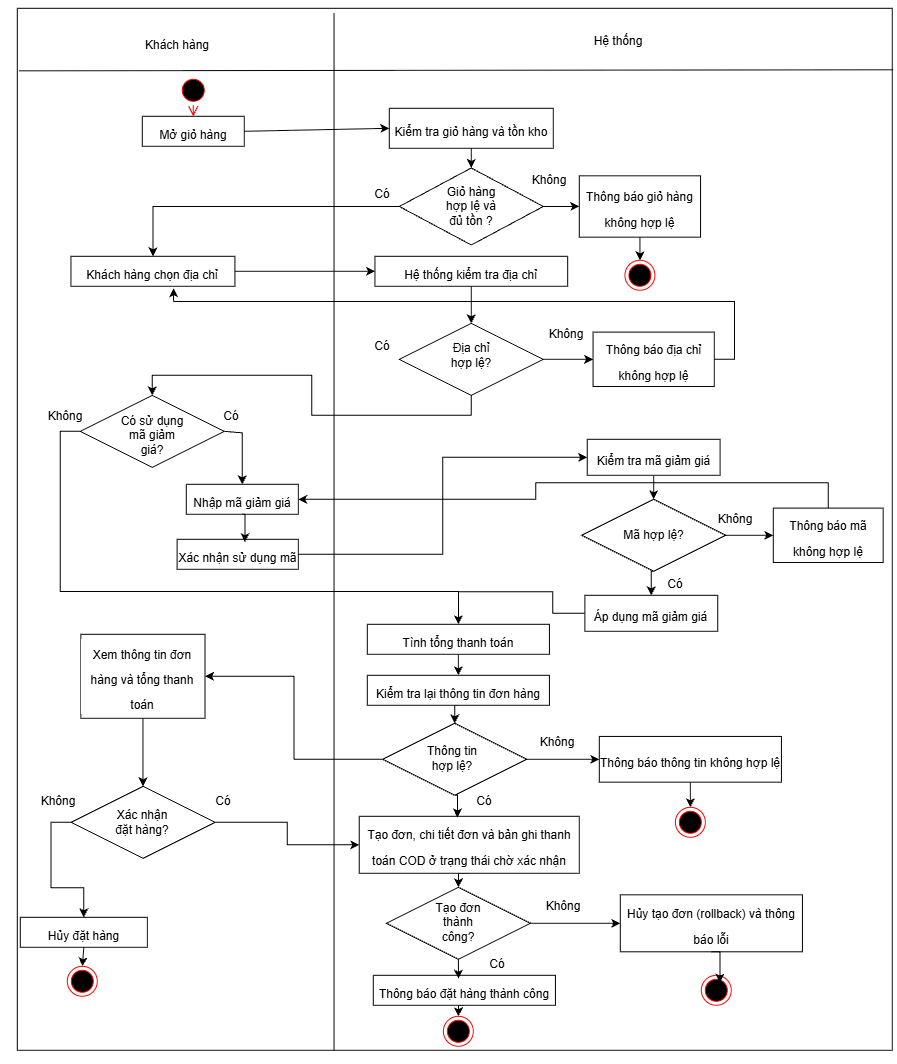
\includegraphics[width=\linewidth,height=0.82\textheight,keepaspectratio]{Images/Activity/da-Đặt hàng COD.drawio.png}
    \caption{Activity Diagram đặt hàng COD}
    \label{fig:activity-cod-checkout}
\end{figure}

Ở bước này hệ thống mới ghi nhận yêu cầu đặt hàng; việc cập nhật tồn kho được thực hiện khi quản trị viên xác nhận xử lý đơn. Sự phân tách này giúp tránh nhầm lẫn giữa thao tác đặt hàng của khách hàng và nghiệp vụ tiếp nhận đơn COD của quản trị viên.

\subsubsection{Hoạt động xử lý và xác nhận đơn COD}

Hình~\ref{fig:activity-cod-confirmation} mô tả UC-AD-06 và UC-AD-07. Sau khi quản trị viên chọn một đơn chờ xác nhận, hệ thống kiểm tra phương thức thanh toán và trạng thái đơn, khóa dữ liệu liên quan rồi kiểm tra lại tồn kho. Việc cập nhật trạng thái đơn, tồn kho, biến động kho và lịch sử xử lý được thực hiện trong cùng một giao dịch. Khi một bước thất bại, hệ thống rollback, giải phóng khóa và ghi log; khi thành công, hệ thống commit và thông báo trạng thái mới cho khách hàng.

\begin{figure}[H]
    \centering
    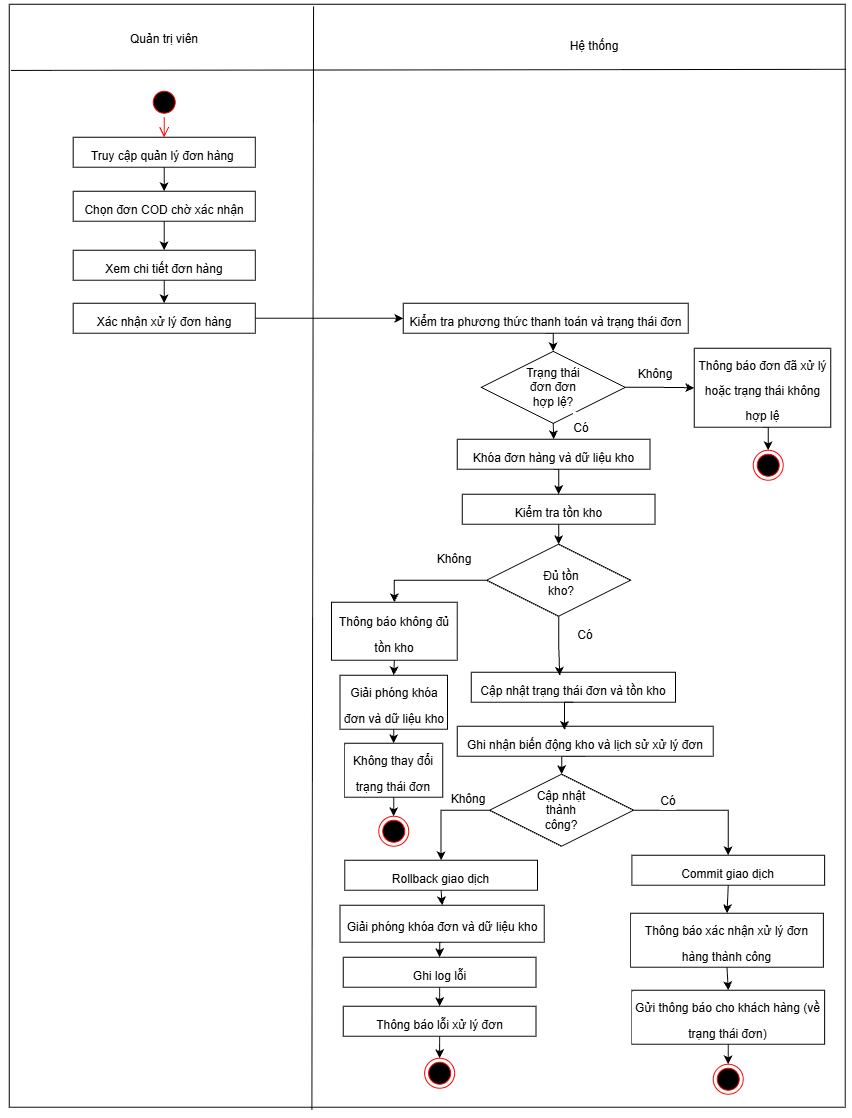
\includegraphics[width=\linewidth,height=0.82\textheight,keepaspectratio]{Images/Activity/da-Xử lý và xác nhận đơn COD.drawio.png}
    \caption{Activity Diagram xử lý và xác nhận đơn COD}
    \label{fig:activity-cod-confirmation}
\end{figure}

Cơ chế khóa và giao dịch bảo đảm hai quản trị viên không đồng thời xác nhận cùng một đơn, đồng thời ngăn trạng thái đơn và số lượng tồn kho bị cập nhật không nhất quán.

\subsubsection{Hoạt động tìm kiếm sản phẩm đa phương thức}

Hình~\ref{fig:activity-multimodal-search} tổng hợp UC-AI-01, UC-AI-02, UC-AI-03 và UC-AI-05. Dựa trên đầu vào, AI Service định tuyến sang tìm kiếm văn bản, hình ảnh hoặc kết hợp. Nhánh văn bản phân tích ý định, trích xuất bộ lọc, tạo text embedding và truy xuất text collection. Nhánh hình ảnh kiểm tra ảnh, sử dụng vùng chọn hoặc ảnh gốc, tạo image embedding và truy xuất image collection.

Với tìm kiếm kết hợp, hai nhánh text và image được xử lý và truy xuất trên các collection tương ứng trước khi hợp nhất danh sách ứng viên. Hệ thống không fusion hai embedding trước khi truy vấn. Sau điểm hợp nhất, các kết quả được lọc theo metadata, rerank nếu tính năng này được bật, rồi đối chiếu với dữ liệu hiện hành từ MySQL để bổ sung giá, khuyến mãi và tồn kho trước khi hiển thị.

\begin{figure}[H]
    \centering
    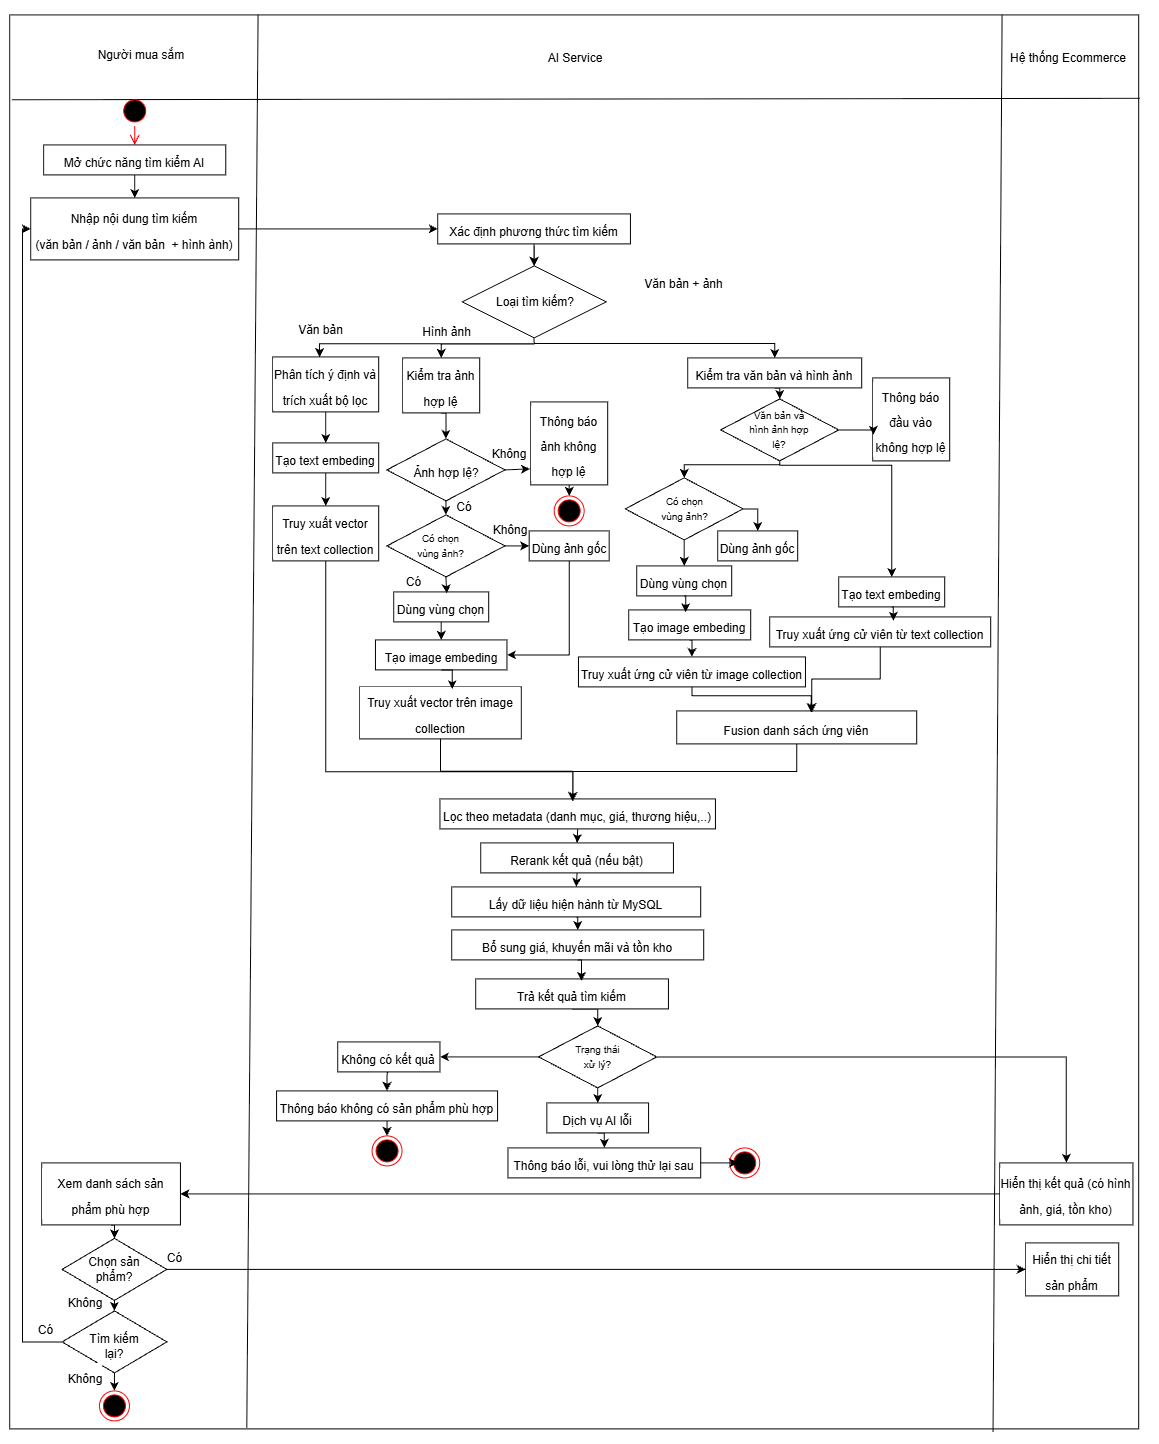
\includegraphics[width=\linewidth,height=0.84\textheight,keepaspectratio]{Images/Activity/da-Tìm kiếm sản phẩm đa phương thức.drawio.png}
    \caption{Activity Diagram tìm kiếm sản phẩm đa phương thức}
    \label{fig:activity-multimodal-search}
\end{figure}

Nếu không có sản phẩm phù hợp, hệ thống trả trạng thái không có kết quả; nếu AI Service gặp lỗi, người dùng nhận thông báo để thử lại. Ở luồng thành công, người dùng có thể xem chi tiết một sản phẩm, thực hiện truy vấn mới hoặc kết thúc phiên tìm kiếm.

\subsubsection{Hoạt động chat tư vấn sản phẩm đa lượt}

Hình~\ref{fig:activity-multiturn-chat} mô tả UC-AI-04 và nhánh phản hồi UC-AI-06. Hệ thống tạo hoặc khôi phục phiên hội thoại, kiểm tra đầu vào rồi chuyển yêu cầu cùng ngữ cảnh đến AI Service. AI Service đọc conversation memory và phân loại ý định thành tìm kiếm sản phẩm, thay đổi điều kiện, hỏi thông tin, small-talk hoặc yêu cầu ngoài phạm vi. Các ý định cần dữ liệu sản phẩm được đưa qua retrieval, lọc metadata và đối chiếu giá, tồn kho hiện hành trước khi tạo câu trả lời có căn cứ.

\begin{figure}[H]
    \centering
    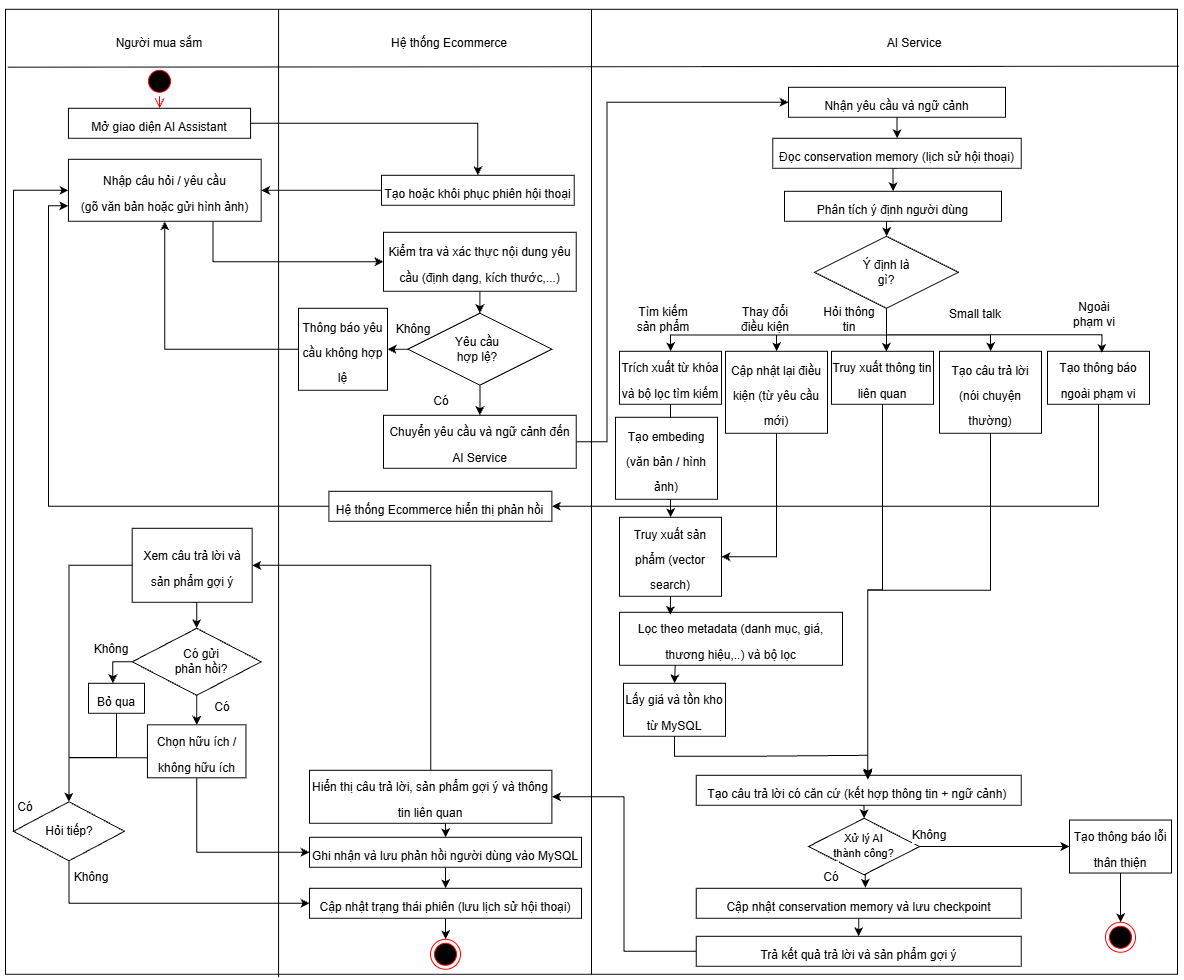
\includegraphics[width=\linewidth,height=0.78\textheight,keepaspectratio]{Images/Activity/da-Chat tư vấn sản phẩm đa lượt.drawio.png}
    \caption{Activity Diagram chat tư vấn sản phẩm đa lượt}
    \label{fig:activity-multiturn-chat}
\end{figure}

Sau mỗi lượt thành công, AI Service cập nhật conversation memory và checkpoint. Người dùng có thể đánh giá câu trả lời là hữu ích hoặc không hữu ích, sau đó tiếp tục đặt câu hỏi trong cùng phiên. Khi người dùng không hỏi tiếp, hệ thống lưu trạng thái phiên và kết thúc; lỗi từ retrieval hoặc mô hình AI được chuyển thành thông báo thân thiện.

\subsubsection{Hoạt động đồng bộ chỉ mục AI}

Hình~\ref{fig:activity-ai-index-sync} mô tả UC-AD-11, UC-AD-12, UC-AI-07 và UC-AI-08. Quản trị viên có thể chọn đồng bộ toàn bộ, tăng dần, theo giới hạn hoặc theo mã sản phẩm. Backend nghiệp vụ kiểm tra quyền và tham số, tạo tác vụ ở trạng thái \texttt{QUEUED}, sau đó chuyển sang \texttt{RUNNING}, lấy dữ liệu từ MySQL và chia danh sách sản phẩm thành các batch.

\begin{figure}[H]
    \centering
    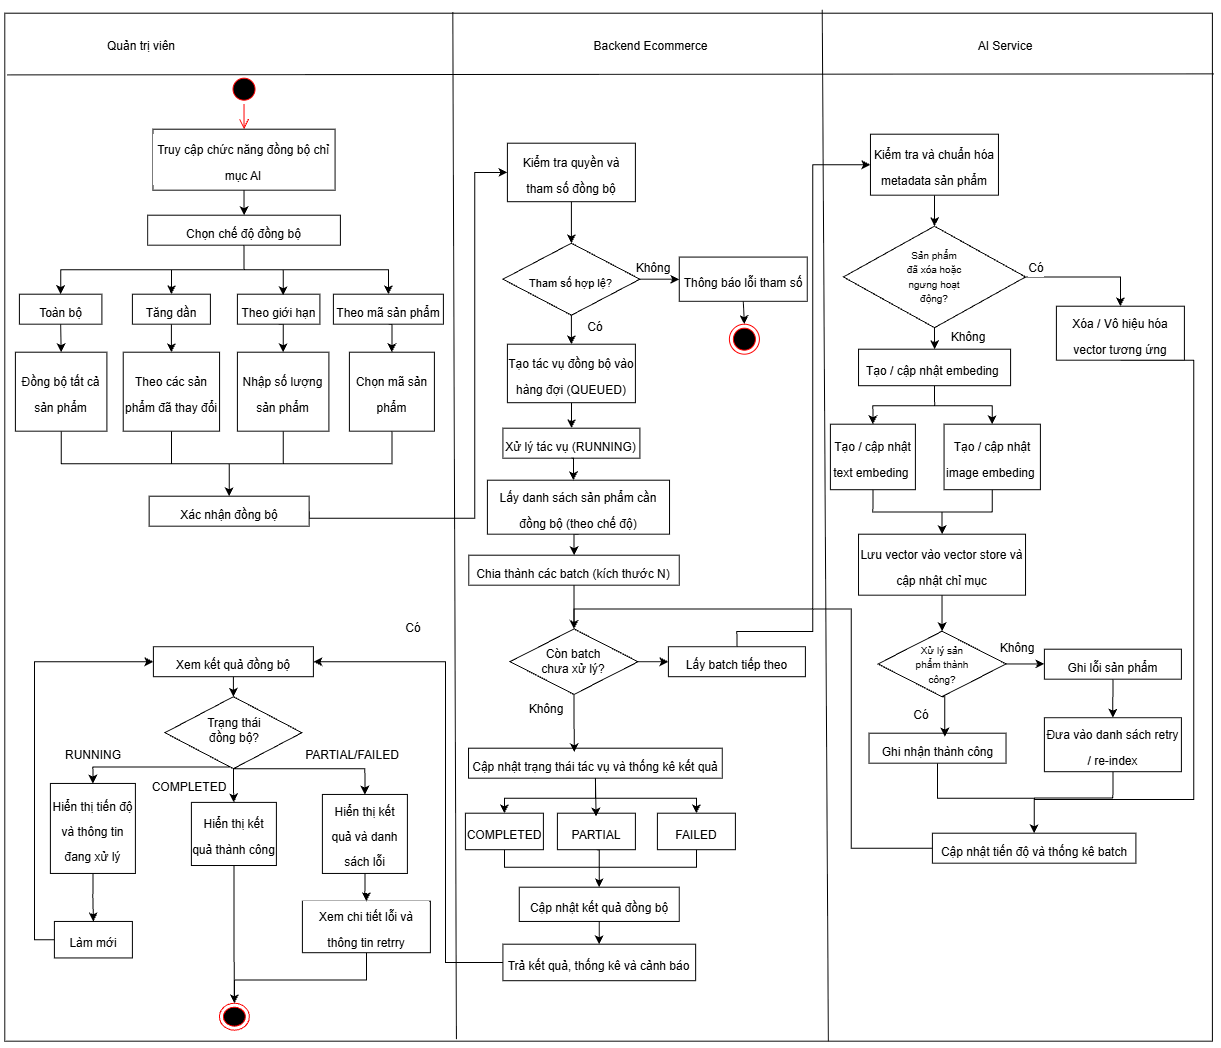
\includegraphics[width=\linewidth,height=0.80\textheight,keepaspectratio]{Images/Activity/da-Đồng bộ chỉ mục AI.drawio.png}
    \caption{Activity Diagram đồng bộ chỉ mục AI}
    \label{fig:activity-ai-index-sync}
\end{figure}

AI Service chuẩn hóa metadata, tạo hoặc cập nhật text embedding và image embedding, rồi lưu vector cùng payload vào vector store. Với sản phẩm đã xóa hoặc ngừng hoạt động, vector tương ứng được xóa hoặc vô hiệu hóa. Kết quả của từng batch được ghi nhận để cập nhật tiến độ; sản phẩm lỗi được đưa vào danh sách retry/re-index mà không làm dừng toàn bộ tác vụ. Khi không còn batch, Backend nghiệp vụ tổng hợp trạng thái \texttt{COMPLETED}, \texttt{PARTIAL} hoặc \texttt{FAILED} và trả thống kê, cảnh báo cho quản trị viên.

\FloatBarrier
\subsection*{Kết chương}

Chương này đã phân tích hệ thống ở các góc nhìn bổ trợ nhau. Ba nhóm Use Case và các bảng đặc tả xác định chức năng, tác nhân, điều kiện và ngoại lệ; năm Activity Diagram mô tả luồng điều khiển, các điểm quyết định và trách nhiệm của những thành phần tham gia các nghiệp vụ tiêu biểu.

Kết quả phân tích bao quát quy trình đặt và xác nhận đơn COD, tìm kiếm đa phương thức, hội thoại tư vấn nhiều lượt và đồng bộ chỉ mục AI. Đây là cơ sở để thiết kế kiến trúc, dữ liệu, giao tiếp dịch vụ và AI retrieval pipeline ở chương tiếp theo.
